\documentclass{article}

\def\npart{III}
\def\nyear{2018}
\def\nterm{Michaelmas}
\def\nlecturer{Dr. S. Barbina}
\def\ncourse{Model Theory}
\usepackage{mathrsfs}
\usepackage{imakeidx}
\usepackage{marginnote}
\ifx \nauthor\undefined
  \def\nauthor{Bhavik Mehta}
\else
\fi

\author{Based on lectures by \nlecturer \\\small Notes taken by \nauthor}
\date{\nterm\ \nyear}
\title{Part \npart\ -- \ncourse}

\usepackage[utf8]{inputenc}
\usepackage{amsmath}
\usepackage{amsthm}
\usepackage{amssymb}
\usepackage{enumerate}
\usepackage{mathtools}
\usepackage{graphicx}
\usepackage[dvipsnames]{xcolor}
\usepackage{tikz}
\usepackage{wrapfig}
\usepackage{centernot}
\usepackage{float}
\usepackage{braket}
\usepackage[hypcap=true]{caption}
\usepackage{enumitem}
\usepackage[colorlinks=true, linkcolor=mblue]{hyperref}
\usepackage[nameinlink,noabbrev]{cleveref}
\usepackage{nameref}
\usepackage[margin=1.5in]{geometry}

% Theorems
\theoremstyle{definition}
\newtheorem*{aim}{Aim}
\newtheorem*{axiom}{Axiom}
\newtheorem*{claim}{Claim}
\newtheorem*{cor}{Corollary}
\newtheorem*{conjecture}{Conjecture}
\newtheorem*{defi}{Definition}
\newtheorem*{eg}{Example}
\newtheorem*{ex}{Exercise}
\newtheorem*{fact}{Fact}
\newtheorem*{law}{Law}
\newtheorem*{lemma}{Lemma}
\newtheorem*{notation}{Notation}
\newtheorem*{prop}{Proposition}
\newtheorem*{question}{Question}
\newtheorem*{rrule}{Rule}
\newtheorem*{thm}{Theorem}
\newtheorem*{assumption}{Assumption}

\newtheorem*{remark}{Remark}
\newtheorem*{warning}{Warning}
\newtheorem*{exercise}{Exercise}

% \newcommand{\nthmautorefname}{Theorem}

\newtheorem{nthm}{Theorem}[section]
\newtheorem{nlemma}[nthm]{Lemma}
\newtheorem{nprop}[nthm]{Proposition}
\newtheorem{ncor}[nthm]{Corollary}
\newtheorem{ndef}[nthm]{Definition}

% Special sets
\newcommand{\C}{\mathbb{C}}
\newcommand{\N}{\mathbb{N}}
\newcommand{\Q}{\mathbb{Q}}
\newcommand{\R}{\mathbb{R}}
\newcommand{\Z}{\mathbb{Z}}

\newcommand{\abs}[1]{\left\lvert #1\right\rvert}
\newcommand{\norm}[1]{\left\lVert #1\right\rVert}
\renewcommand{\vec}[1]{\boldsymbol{\mathbf{#1}}}

\let\Im\relax
\let\Re\relax

\DeclareMathOperator{\Im}{Im}
\DeclareMathOperator{\Re}{Re}
\DeclareMathOperator{\id}{id}

\definecolor{mblue}{rgb}{0., 0.05, 0.6}

\makeindex[intoc]
\usetikzlibrary{intersections, decorations.pathmorphing}

% preamble

\reversemarginpar

\let\oldmodels\models
\let\models\vDash
\let\nModels\nvDash

\setcounter{section}{-1}

\DeclareMathOperator{\Mod}{Mod}
\DeclareMathOperator{\Aut}{Aut}
\DeclareMathOperator{\Th}{Th}
\DeclareMathOperator{\dom}{dom}
\DeclareMathOperator{\img}{img}
\DeclareMathOperator{\tp}{tp}
\DeclareMathOperator{\qftp}{qftp}
\DeclareMathOperator{\dcl}{dcl}
\DeclareMathOperator{\acl}{acl}
\DeclareMathOperator{\cof}{cof}
\DeclarePairedDelimiter\ceil{\lceil}{\rceil}
\DeclarePairedDelimiter\floor{\lfloor}{\rfloor}

\newtheorem{nremark}[nthm]{Remark}
\newtheorem{nexample}[nthm]{Example}
\newtheorem{nexercise}[nthm]{Exercise}
\newtheorem{nfact}[nthm]{Fact}
\newtheorem{nnotation}[nthm]{Notation}

\newcommand{\named}[1]{\textbf{#1}\index{#1}}
\newcommand{\bonusnamed}[1]{\textbf{#1}\index{#1@*#1}}
\newcommand{\M}{\mathcal{M}}
\renewcommand{\N}{\mathcal{N}}
\newcommand{\U}{\mathcal{U}}

% and here we go!

\begin{document}
\maketitle

\tableofcontents

\clearpage
\section{Introduction}
Model\marginnote{\emph{Lecture 1}}[0cm] theory is a part of logic that began by looking at algebraic objects such as groups and combinatorial objects such like graphs, described in formal language.
The basic question in model theory is: `how powerful is our description of these objects to pin them down'?
In Logic and Set Theory, the focus was on what was provable from a theory and language, but here we focus on whether or not a model exists.

\section{Languages and structures}
\begin{ndef}[Language]\label{def:1.1}\hypertarget{def:lang}
  A \named{language} $L$ consists of
  \begin{enumerate}[label=(\roman*)]
    \item a set $\mathscr{F}$ of function symbols, and for each $f \in \mathscr{F}$ a positive integer $m_f$ the \named{arity} of $f$.
    \item a set $\mathscr{R}$ of relation symbols, and for each $R \in \mathscr{R}$, a positive integer $m_R$.
    \item a set $\mathscr{C}$ of constant symbols.
  \end{enumerate}
  Note: each of $\mathscr{F}, \mathscr{R}$ and $\mathscr{C}$ can be empty.
\end{ndef}
\begin{eg}
  \hypertarget{def:lgp}Take $L = \{\{\cdot , ^{-1}\}, \{1\}\}$, for $\cdot$ a binary function and $^{-1}$ an unary function, $1$ a constant. This is the \hyperlink{def:lang}{language} of groups, call it $L_{\text{gp}}$.
  Also, $L_{\text{lo}} = \{<\}$ a single binary relation, for linear orders.
\end{eg}

\begin{ndef}[$L$-structure]\label{def:1.2}\index{structure}\hypertarget{def:str}
  Given a \hyperlink{def:lang}{language} $L$, say, an \textbf{$L$-structure} consists of
  \begin{enumerate}[label=(\roman*)]
    \item a set $M$, the \named{domain}
    \item for each $f \in \mathscr{F}$, a function $f^\mathcal{M} : M^{m_f} \to M$.
    \item for each $R \in \mathscr{R}$, a relation $R^\mathcal{M} \subseteq M^{m_R}$.
    \item for each $c \in \mathscr{C}$, an element $c^\mathcal{M} \in M$.
  \end{enumerate}
  $f^M, R^M, c^M$ are the \named{interpretations} of $f,R,c$ respectively.
\end{ndef}
\begin{nremark}\label{rem:1.3}
  We often fail to distinguish between the \hyperlink{def:lang}{symbols} in $L$ and their \hyperlink{def:str}{interpretations} in a \hyperlink{def:str}{structure}, if the interpretations are clear from the context.
\end{nremark}

We may write $\mathcal{M} = \langle M, \mathscr{F}, \mathscr{R}, \mathscr{C} \rangle$.

\begin{nexample}\label{eg:1.4}\leavevmode
  \begin{enumerate}[label=(\alph*)]
    \item $\mathcal{R} = \langle \mathbb{R}^+, \{\cdot, ^{-1}\}, 1 \rangle$ is an \hyperlink{def:lgp}{$L_{\text{gp}}$}-\hyperlink{def:str}{structure}.
    \item $\mathcal{Z} = \langle \mathbb{Z}, \{+, -\}, 0 \rangle$ is an $L_{\text{gp}}$-structure.
    \item $\mathcal{Q} = \langle \mathbb{Q}, < \rangle$ is an \hyperlink{def:lgp}{$L_{\text{lo}}$}-structure.
  \end{enumerate}
\end{nexample}
\begin{ndef}[Embedding]\label{def:1.5}\hypertarget{def:embedding}
  Let $L$ be a \hyperlink{def:lang}{language}, let $\mathcal{M}, \mathcal{N}$ be \hyperlink{def:str}{$L$-structures}.
  An \named{embedding} of $\mathcal{M}$ into $\mathcal{N}$ is a one-to-one mapping $\alpha: M \to N$ such that
  \begin{enumerate}[label=(\roman*)]
    \item for all $f \in \mathscr{F}$, and $a_1, \dotsc, a_{m_f} \in M$,
      \begin{equation*}
        \alpha(f^\mathcal{M}(a_1, \dotsc, a_{m_f})) = f^\mathcal{N}(\alpha(a_1), \dotsc, \alpha(a_{m_f})) \end{equation*}
      \begin{center}
        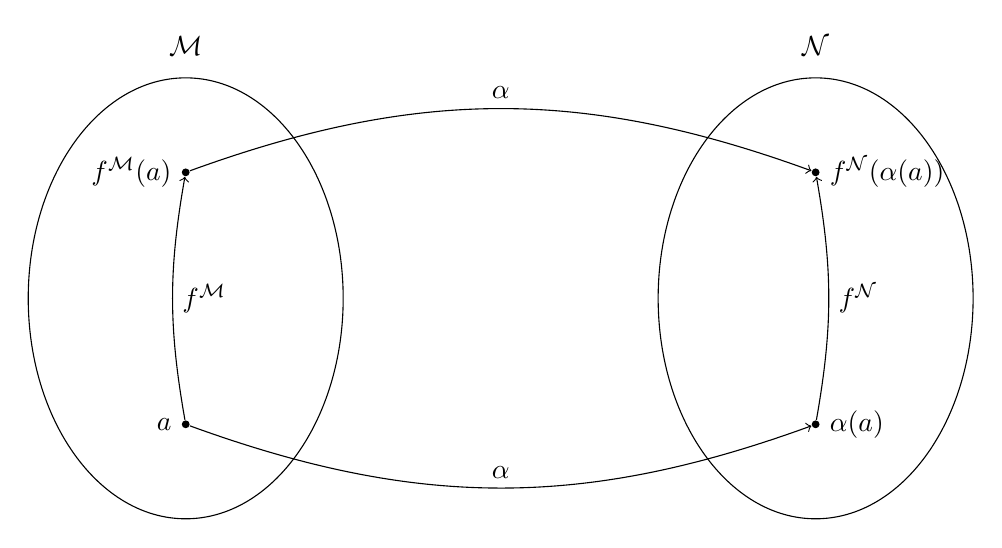
\begin{tikzpicture}[scale=2]
          \node at (-2, 1.6) {$\mathcal{M}$};
          \node at (2, 1.6) {$\mathcal{N}$};
          \draw (-2, 0) circle [x radius=10mm, y radius=14mm];
          \node [circle, inner sep=1pt, fill=black, label=left:$a$] (a) at (-2, -0.8) {};
          \node [circle, inner sep=1pt, fill=black, label=left:$f^\mathcal{M}(a)$] (fa) at (-2, 0.8) {};
          \draw (2, 0) circle [x radius=10mm, y radius=14mm];
          \node [circle, inner sep=1pt, fill=black, label=right:$\alpha(a)$] (aa) at (2, -0.8) {};
          \node [circle, inner sep=1pt, fill=black, label=right:$f^\mathcal{N}(\alpha(a))$] (faa) at (2, 0.8) {};
          \draw [->] (a) to [bend right=20] node[above]{$\alpha$} (aa);
          \draw [->] (fa) to [bend left=20] node[above]{$\alpha$} (faa);
          \draw [->] (a) to [bend left=10] node[right]{$f^\mathcal{M}$} (fa);
          \draw [->] (aa) to [bend right=10] node[right]{$f^\mathcal{N}$} (faa);
        \end{tikzpicture}
      \end{center}
    \item for all $R \in \mathscr{R}$, and $a_1, \dotsc, a_{m_R} \in M$
      \begin{equation*}
        (a_1, \dotsc, a_{m_R}) \in R^\mathcal{M} \iff (\alpha(a_1), \dotsc, \alpha(a_{m_R})) \in R^\mathcal{N}
      \end{equation*}
    \item for all $c \in \mathscr{C}$, $\alpha(c^\mathcal{M}) = c^\mathcal{N}$.
  \end{enumerate}
  \hypertarget{def:iso}An \named{isomorphism} of $\mathcal{M}$ into $\mathcal{N}$ is a surjective embedding (onto), written $\M \simeq \N$.
\end{ndef}

\begin{nexercise}\label{ex:1.6}
  Let $G_1, G_2$ be groups, regarded as \hyperlink{def:lgp}{$L_{\text{gp}}$}-structures.
  Check that $G_1 \simeq G_2$ in the usual algebra sense if and only if there is an \hyperlink{def:iso}{isomorphism} $\alpha: G_1 \to G_2$ in the sense of \cref{def:1.5}.
\end{nexercise}

\clearpage
\section{Review: Terms, formulae and their interpretations}
In addition to the \hyperlink{def:lang}{symbols} of $L$, we also have
\begin{enumerate}[label=(\roman*)]
  \item infinitely many variables $\{x_i\}_{i \in I}$
  \item logical connectives $\wedge, \neg$ (also expresses $\vee, \implies, \iff$)
  \item quantifier $\exists$ (also expresses $\forall$)
  \item $(\phantom{-},\phantom{-})$
  \item equality symbol $=$
\end{enumerate}

\begin{ndef}[\hypertarget{def:lterm}{$L$-terms}]\label{def:2.1}
  \index{term}\textbf{$L$-terms} are defined recursively as follows:
  \begin{itemize}[label=--]
    \item any variable $x_i$ is a term
    \item any constant symbol is a term
    \item for any $f \in \mathscr{F}$, $f(t_1, \dotsc, t_{m_f})$ for any terms $t_1, \dotsc, t_{m_f}$ is a term
    \item nothing else is a term
  \end{itemize}
\end{ndef}

Notation: we write $t(x_1, \dotsc, x_m)$ to mean that the variables appearing in $t$ are among $x_1, \dotsc, x_m$.
\begin{eg}
  \marginnote{\emph{Lecture 2}}[0cm]
  Take $\mathcal{R} = \langle \mathbb{R}^*, \{\cdot, ^{-1}\}, 1 \rangle$.
  Then $\cdot ( \cdot(x_1, x_2), x_3)$ is a \hyperlink{def:lterm}{term}, usually written $(x_1 \cdot x_2) \cdot x_3$.
  Also, $(\cdot (1, x_1))^{-1}$ is a \hyperlink{def:lterm}{term}, written $(1\cdot x)^{-1}$
\end{eg}
\begin{ndef}\label{def:2.2}\hypertarget{def:funcAssign}
  If $\mathcal{M}$ is an \hyperlink{def:str}{$L$-structure}, to each \hyperlink{def:lterm}{$L$-term} $t(x_1, \dotsc, x_k)$ we assign a function
  a function $t^\mathcal{M}: M^k \to M$ defined as follows:
  \begin{enumerate}[label=(\roman*)]
    \item If $t = x_i$, $t^\mathcal{M}[a_1, \dotsc, a_k] = a_i$
    \item If $t = c$, $t^\mathcal{M}[a_1, \dotsc, a_k] = c^\mathcal{M}$.
    \item If $t = f(t_1(x_1, \dotsc, x_k), \dotsc, t_{m_f}(x_1, \dotsc, x_k))$, then
      \begin{equation*}
        t^\mathcal{M}(a_1, \dotsc, a_k) = f^\mathcal{M}(t_1^\mathcal{M}(a_1, \dotsc, a_k), \dotsc, t^\mathcal{M}_{m_f}(a_1, \dotsc, a_k)).
      \end{equation*}
  \end{enumerate}
\end{ndef}

Notice in $\hyperlink{def:lgp}{L_{\text{gp}}}$, the term $x_2 \cdot x_3$ can be described as $t_1(x_1, x_2, x_3)$ or $t_2(x_1, x_2, x_3, x_4)$, or infinitely many other ways.
In these cases, $t_1$ is \hyperlink{def:funcAssign}{assigned} to $t_1^\mathcal{M}: M^3 \to M$, with $(a_1, a_2, a_3) \mapsto (a_2, a_3)$, and $t_2$ is assigned to $t_2^\mathcal{M} : M^4 \to M$, with $(a_1, a_2, a_3, a_4) \mapsto a_2 \cdot a_3$.
\begin{nfact}\label{fact:2.3}
  Let $\mathcal{M}, \mathcal{N}$ be \hyperlink{def:str}{$L$-structures}, and let $\alpha: \mathcal{M} \to \mathcal{N}$ be an \hyperlink{def:embedding}{embedding}.
  For any \hyperlink{def:lterm}{$L$-term} $t(x_1, \dotsc, x_k)$ and $a_1, \dotsc, a_k \in M$ we have
  \begin{equation*}
    \alpha(\hyperlink{def:funcAssign}{t^\mathcal{M}}(a_1, \dotsc, a_k)) = t^\mathcal{N}(\alpha(a_1), \dotsc, \alpha(a_k))
  \end{equation*}
\end{nfact}
\begin{proof}
  By induction on the complexity of $t$. Let $\bar{a} = (a_1, \dotsc, a_k)$ and $\bar{x} = (x_1, \dotsc, x_k)$.
  Then
  \begin{enumerate}[label=(\roman*)]
    \item if $t = x_i$, then $t^\mathcal{M}(\bar{a}) = a_i$, and $t^\mathcal{N}(\alpha(a_1), \dotsc, \alpha(a_k)) = \alpha(a_i)$, so the conclusion holds.
    \item if $t = c$ a constant, then $t^\mathcal{M}(\bar{a}) = c^\mathcal{M}$, and $t^\mathcal{N}(\alpha(\bar{a})) = c^\mathcal{N}$, and $\alpha(c^\mathcal{M}) = c^\mathcal{N}$, as required.
    \item if $t = f(t_1(\bar{x}),\dotsc, t_{m_f}(\bar{x}))$, then
      \begin{equation*}
        \alpha(f^\mathcal{M}(t_1^\mathcal{M}(\bar{a}), \dotsc, t_{m_f}^\mathcal{M}(\bar{a}))) = f^\mathcal{N}(\alpha(t_1^\mathcal{M}(\bar{a})), \dotsc, \alpha(t_{m_f}^\mathcal{M}(\bar{a})))
      \end{equation*}
      since $\alpha$ is an \hyperlink{def:embedding}{embedding}.
      $t_1(\bar{x}), \dotsc, t_{m_f}(\bar{x})$ have lower complexity than $t$, so inductive hypothesis applies. \qedhere
  \end{enumerate}
\end{proof}
\begin{nexercise}\label{ex:2.4}
  Conclude the proof of \cref{fact:2.3}.
\end{nexercise}
\begin{ndef}[Atomic formula]\label{def:2.5}\index{formula!atomic}\hypertarget{def:atomform}
  The set of \named{atomic formulas} of $L$ is defined as follows
  \begin{enumerate}[label=(\roman*)]
    \item if $t_1, t_2$ are $L$-terms, then $t_1 = t_2$ is an atomic formula
    \item if $R$ is a relation symbol and $t_1, \dotsc, t_{m_R}$ are terms, then $R(t_1, \dotsc, t_{m_R})$ is an atomic formula
    \item nothing else is an atomic formula.
  \end{enumerate}
\end{ndef}
\begin{ndef}[Formula]\label{def:2.6}\index{formula}\hypertarget{def:form}
  The set of \textbf{$L$-formulas} is defined as follows
  \begin{enumerate}[label=(\roman*)]
    \item any \hyperlink{def:atomform}{atomic formula} is an $L$-formula
    \item if $\phi$ is an $L$-formula, then so is $\neg \phi$
    \item if $\phi$ and $\psi$ are $L$-formulas, then so is $\phi \wedge \psi$
    \item if $\phi$ is an $L$-formula, for any $i \geq 1$, $\exists x_i \; \phi$ is an $L$-formula
    \item nothing else is an $L$-formula
  \end{enumerate}
\end{ndef}
\begin{eg}
  In $\hyperlink{def:lgp}{L_{\text{gp}}}$, $x_1 \cdot x_1 = x_2$ and $x_1 \cdot x_2 = 1$ are \hyperlink{def:form}{atomic formulas}, and $\exists x_1 \; (x_1 \cdot x_2) = 1$ is an $L_{\text{gp}}$-formula.
\end{eg}
\hypertarget{def:free}A variable occurs freely in a formula if it does not occur within the scope of a quantifier $\exists$ (the variable is \named{free}). Otherwise the variable is \named{bound}. For instance, in $\exists x_1 \; (x_1 \cdot x_2) = 1$, $x_1$ is bound and $x_2$ is free.

\textbf{Important convention:} no variable occurs both \hyperlink{def:free}{freely} and as a bound variable in the same formula.

\hypertarget{def:sentence}A \named{sentence} is a \hyperlink{def:form}{formula} with no \hyperlink{def:free}{free} variables.
\begin{equation*}
\exists x_1 \exists x_2 \; (x_1 \cdot x_2 = 1)
\end{equation*}
is an \hyperlink{def:lgp}{$L_{\text{gp}}$}-sentence.
Notation: $\phi(x_1, \dotsc, x_k)$ means that the free variables in $\phi$ are among $x_1, \dotsc, x_k$.

\begin{ndef}[$\models$]\label{def:2.7}\index{$\models$}\hypertarget{def:models}
  Let $\phi(x_1, \dotsc, x_k)$ be an \hyperlink{def:form}{$L$-formula}, let $\mathcal{M}$ be an \hyperlink{def:str}{$L$-structure}, and let $\bar{a} = (a_1, \dotsc, a_k)$ be elements of $M$.
  We define $\mathcal{M} \models \phi(\bar{a})$ recursively as follows.
  \begin{enumerate}[label=(\roman*)]
    \item if $\phi$ is $t_1 = t_2$, then $\mathcal{M} \models \phi(\bar{a})$ if and only if $\hyperlink{def:funcAssign}{t_1^\mathcal{M}}(\bar{a}) = t_2^\mathcal{M}(\bar{a})$.
    \item if $\phi$ is $R(t_1, \dotsc, t_{m_k})$ then $\mathcal{M} \models \phi(\bar{a})$ iff
      \begin{equation*}
        (t_1^\mathcal{M}(\bar{a}),\dotsc,t_{m_k}^\mathcal{M}(\bar{a})) \in R^\mathcal{M}.
      \end{equation*}
    \item if $\phi$ is $\psi \wedge \chi$, then $\mathcal{M} \models \phi(\bar{a})$ iff $\mathcal{M} \models \psi(\bar{a})$ and $\mathcal{M} \models \chi(\bar{a})$.
    \item if $\phi = \neg \psi$ then $\mathcal{M} \models \phi(\bar{a})$ iff $\mathcal{M} \nModels \psi(\bar{a})$. (this is well-defined since $\psi(\bar{a})$ is shorter than $\phi(\bar{a})$)
    \item if $\phi$ is $\exists x_j\ \chi(x_1, \dotsc, x_k, x_j)$ (where $x_j \neq x_i$ for $i = 1, \dotsc, k$).
      Then $\mathcal{M} \models \phi(\bar{a})$ iff there is $b \in \mathcal{M}$ such that $\mathcal{M} \models \chi(a_1, \dotsc, a_k, b)$.
  \end{enumerate}
\end{ndef}
\begin{eg}
  For $\mathcal{R} = \langle \mathbb{R}^*,\cdot, ^{-1}, 1\rangle$, if $\phi(x_1) = \exists x_2 \; (x_2 \cdot x_2) = x_1$ then $\mathcal{R} \hyperlink{def:models}{\models} \phi(1)$ but $\mathcal{R} \nModels \phi(-1)$.
\end{eg}
\begin{nnotation}[Useful abbreviations]\label{not:2.8}
  We write
  \begin{itemize}[label=--]
    \item $\phi \vee \psi$ for $\neg(\neg\phi \wedge \neg\psi)$
    \item $\phi \to \psi$ for $\neg \phi \vee \psi$
    \item $\phi \leftrightarrow \psi$ for $(\phi \to \psi) \wedge (\psi \to \phi)$
    \item $\forall x_i\ \phi$ for $\neg \exists x_i\ (\neg \phi)$
  \end{itemize}
\end{nnotation}
\begin{nprop}\label{prop:2.9}
  Let $\mathcal{M}, \mathcal{N}$ be \hyperlink{def:str}{$L$-structures}, let $\alpha: \mathcal{M} \to \mathcal{N}$ be an \hyperlink{def:embedding}{embedding}.
  Let $\phi(\bar{x})$ be \hyperlink{def:atomform}{atomic} and $\bar{a} \in M^{|\bar{x}|}$, then
  \begin{equation*}
    M \hyperlink{def:models}{\models} \phi(\bar{a}) \iff \mathcal{N} \models \phi(\alpha(\bar{a})).
  \end{equation*}
\end{nprop}

Question: If $\phi$ is an \hyperlink{def:form}{$L$-formula}, not necessarily \hyperlink{def:atomform}{atomic}, does \cref{prop:2.9} hold?

\begin{proof}[Proof of \cref{prop:2.9}]
  Cases:\marginnote{\emph{Lecture 3}}[0cm]
  \begin{enumerate}[label=(\roman*)]
    \item $\phi(\bar{x})$ is of the form $t_1(\bar{x}) = t_2(\bar{x})$ where $t_1,t_2$ are terms.
      (Exercise: complete this case, using \cref{fact:2.3})
    \item $\phi(\bar{x})$ is of the form $R(t_1(\bar{x}), \dotsc, t_{m_R}(\bar{x}))$.
      Then $\mathcal{M} \hyperlink{def:models}{\models} R(t_1(\bar{a}), \dotsc, t_{m_R}(\bar{a}))$ if and only if...
      (Exercise: complete this case)
  \end{enumerate}
\end{proof}
\begin{nexercise}\label{ex:2.10}
  Show that \cref{prop:2.9} holds if $\phi(\bar{x})$ is a formula without quantifiers (a quantifier-free formula).
\end{nexercise}
\begin{nexample}\label{ex:2.11}
  Do \hyperlink{def:embedding}{embeddings} preserve \emph{all} \hyperlink{def:form}{formulas}? No.
  Take $\mathcal{Z} = (\mathbb{Z}, <)$ and $\mathcal{Q} = (\mathbb{Q}, <)$ an \hyperlink{def:lgp}{$L_{\text{lo}}$}-\hyperlink{def:str}{structure}.
  Then $\alpha: \mathbb{Z} \to \mathbb{Q}$ (inclusion) is an embedding, but
  \begin{gather*}
    \phi(x_1, x_2) = \exists x_3\,(x_1 < x_3 \wedge x_3 < x_2). \\
    \mathcal{Q} \hyperlink{def:models}{\models} \phi(1,2) \text{ but } \mathcal{Z} \nModels \phi(1,2).
  \end{gather*}
\end{nexample}
\begin{nfact}\label{fact:2.12}
  Let $\alpha: \mathcal{M} \to \mathcal{N}$ be an \hyperlink{def:iso}{isomorphism}.
  Then if $\phi(\bar{x})$ is an \hyperlink{def:form}{$L$-formula} and $\bar{a} \in M^{|\bar{x}|}$, then
  \begin{equation*}
    \mathcal{M} \hyperlink{def:models}{\models} \phi(\bar{a}) \iff \mathcal{M} \models \phi(\alpha(\bar{a})).
  \end{equation*}
\end{nfact}
\begin{proof}
  Exercise.
\end{proof}

\clearpage
\section{Theories and elementarity}
Throughout, $L$ is a \hyperlink{def:lang}{language}, $\mathcal{M}, \mathcal{N}$ are \hyperlink{def:str}{$L$-structures}.
\begin{ndef}[$L$-theory]\label{def:3.1}\index{theory}\hypertarget{def:ltheory}
  An \textbf{$L$-theory} $T$ is a set of \hyperlink{def:sentence}{$L$-sentences}.
  \hypertarget{def:model}$\mathcal{M}$ is a \named{model} of $T$ if $\mathcal{M} \hyperlink{def:models}{\models} \sigma$ for all $\sigma \in T$. We write $\mathcal{M} \models T$.
  The class of all the models of $T$ is written $\Mod(T)$.
  The theory of $\mathcal{M}$ is the set
  \begin{equation*}
    \Th(\mathcal{M}) = \set{\sigma | \sigma \text{ is an } L\text{-\hyperlink{def:sentence}{sentence} and } \mathcal{M} \models \sigma}.
  \end{equation*}
\end{ndef}
\begin{nexample}\label{eg:3.2}
  Let $T_{\text{gp}}$ be the set of \hyperlink{def:lgp}{$L_{\text{gp}}$}-\hyperlink{def:sentence}{sentences}
  \begin{enumerate}[label=(\roman*)]
    \item $\forall x_1 x_2 x_3\, (x_1 \cdot (x_2 \cdot x_3) = (x_1 \cdot x_2) \cdot x_3)$
    \item $\forall x_1\, (x_1 \cdot 1 = 1 \cdot x_1 = x_1)$
    \item $\forall x_1\,(x_1 \cdot x_1^{-1} = x_1^{-1} \cdot x_1 = 1)$
  \end{enumerate}
\end{nexample}
Clearly for a group $G$, $G \hyperlink{def:models}{\models} T_{\text{gp}}$. For a specific $G$, clearly $\hyperlink{def:ltheory}{\Th(G)}$ is larger than $T_{\text{gp}}$!

\begin{ndef}[Elementarily equivalent]\label{def:3.3}
  \hypertarget{def:eleq}Say $\mathcal{M}$ and $\mathcal{N}$ are \named{elementarily equivalent} if $\Th(\mathcal{M}) = \Th(\mathcal{N})$.
  We write $\mathcal{M} \equiv \mathcal{N}$.
\end{ndef}
Clearly if $\hyperlink{def:iso}{\mathcal{M} \simeq \mathcal{N}}$, then \hyperlink{def:eleq}{$\mathcal{M} \equiv \mathcal{N}$} but if $\mathcal{M}$ and $\mathcal{N}$ are not \hyperlink{def:iso}{isomorphic}, establishing whether $\mathcal{M} \equiv \mathcal{N}$ can be highly non-trivial!

We'll see $(\mathbb{Q}, <) \equiv (\mathbb{R}, <)$ as \hyperlink{def:lgp}{$L_{\text{lo}}$}-\hyperlink{def:str}{structures}.
\begin{ndef}[Elementary substructure]\label{def:3.4}\leavevmode
  \begin{enumerate}[label=(\roman*)]
    \item \index{elementary embedding}\index{elementary map}\hypertarget{def:el}an \hyperlink{def:embedding}{embedding} $\beta: \mathcal{M} \to \mathcal{N}$ is \named{elementary} if for all \hyperlink{def:form}{formulas} $\phi(\bar{x})$ and $\bar{a} \in M^{|\bar{x}|}$,
      \begin{equation*}
        \mathcal{M} \hyperlink{def:models}{\models} \phi(\bar{a}) \iff \mathcal{N} \models \phi(\beta(\bar{a})).
      \end{equation*}
    \item \index{substructure}\hypertarget{def:subs}if $M \subseteq N$ and $\operatorname{id}: \mathcal{M} \to \mathcal{N}$ is an embedding, then $\mathcal{M}$ is said to be a \named{substructure} of $\mathcal{N}$, written $\mathcal{M} \subseteq \mathcal{N}$.
    \item \index{elementary substructure}\hypertarget{def:elsubs}if $M \subseteq N$ and $\operatorname{id}: \mathcal{M} \to \mathcal{N}$ is an elementary embedding, then $\mathcal{M}$ is said to be an \named{elementary substructure} of $\mathcal{N}$, written $\mathcal{M} \preccurlyeq \mathcal{N}$.
  \end{enumerate}
\end{ndef}
\begin{nexample}\label{eg:3.5}
  Consider $\mathcal{M} = [0,1] \subseteq \mathbb{R}$, an \hyperlink{def:lgp}{$L_{\text{lo}}$}-\hyperlink{def:str}{structure}, where $<$ is the usual order, and $\mathcal{N} = [0,2] \subseteq \mathbb{R}$ in the same way.
  Then $\hyperlink{def:iso}{\mathcal{M} \simeq \mathcal{N}}$ as $L_{\text{lo}}$-structures.

  Is \hyperlink{def:eleq}{$\mathcal{M} \equiv \mathcal{N}$}? Yes: they are isomorphic!

  Is $\hyperlink{def:subs}{\mathcal{M} \subseteq \mathcal{N}}$? Yes (the ordering $<$ coincides on $\mathcal{M}$ and $\mathcal{N}$.)

  But $\hyperlink{def:elsubs}{\mathcal{M} \not\preccurlyeq \mathcal{N}}$, since if $\phi(x) = \exists y \; (x < y)$, then
  \begin{equation*}
    \mathcal{N} \models \phi(1)\quad\text{and}\quad\mathcal{M} \nModels \phi(1).
  \end{equation*}
\end{nexample}
\begin{ndef}[Parameter]\label{def:3.6}
  \hypertarget{def:la}Let $\mathcal{M}$ be an $L$-\hyperlink{def:str}{structure}, $A \subseteq M$, then define
  \begin{equation*}
    L(A) \coloneqq L \cup \set{c_a | a \in A}
  \end{equation*}
  for $c_a$ each constant symbols.
  An \hyperlink{def:str}{interpretation} of $\mathcal{M}$ as an $L$-structure extends to an interpretation of $\mathcal{M}$ as an $L(A)$-structure in the obvious way ($c_a^\mathcal{M} = a$).
  The elements of $A$ are called \named{parameters}.
  \hypertarget{def:eleqa}If $\mathcal{M}, \mathcal{N}$ are $L$-structures and $A \subseteq M \cap N$, then we write $\mathcal{M} \equiv_A \mathcal{N}$ when $\mathcal{M}, \mathcal{N}$ satisfy exactly the same $L(A)$-\hyperlink{def:sentence}{sentences}.
\end{ndef}

\begin{nexercise}\label{ex:3.7}
  \marginnote{\emph{Lecture 4}}[0cm]
  $ \hyperlink{def:elsubs}{\mathcal{M}\preccurlyeq \mathcal{N}} \iff \hyperlink{def:eleqa}{\mathcal{M} \equiv_M \mathcal{N}}$ (where $M$ is the \hyperlink{def:str}{domain} of $\mathcal{M}$).
\end{nexercise}
\begin{nlemma}[Tarski-Vaught test]\label{lem:3.8}
  Let $\mathcal{N}$ be an \hyperlink{def:str}{$L$-structure}, let $A \subseteq N$. The following are equivalent:
  \begin{enumerate}[label=(\roman*)]
    \item $A$ is the \hyperlink{def:str}{domain} of a structure $\mathcal{M}$ such that $\hyperlink{def:elsubs}{\mathcal{M} \preccurlyeq \mathcal{N}}$.
    \item for every $L(A)$-formula $\phi(x)$ with one free variable, if $\mathcal{N} \hyperlink{def:models}{\models} \exists x \; \phi(x)$, then $\mathcal{N} \models \phi(b)$ for some $b \in A$.
  \end{enumerate}
\end{nlemma}
\begin{proof}\leavevmode
  \begin{description}
    \item [(i) $\Rightarrow$ (ii)] Suppose $\mathcal{N} \models \phi(x)$.
      Then by elementarity, $\mathcal{M} \models \exists x \; \phi(x)$, and so $\mathcal{M} \models \exists x \; \phi(x)$ for $b \in \mathcal{M}$, so again by elementarity $\mathcal{N} \models \phi(b)$.
    \item [(ii) $\Rightarrow$ (i)] First we prove that $A$ is the domain $\mathcal{M} \subseteq \mathcal{N}$.
      By exercise 4 on sheet 1, it is enough to check:
      \begin{enumerate}[label=(\alph*)]
        \item for each constant $c$, $c^\mathcal{N} \in A$.
        \item for each function symbol $f$, $f^{\mathcal{N}}(\bar{a}) \in A$ (for all $\bar{a} \in A^{m_f}$).
      \end{enumerate}
      For (a), use property (ii) with $\exists x\; (x = c)$. For (b) use property (ii) with $\exists x\; (f(\bar{a}) = x)$.

      So we now have $\mathcal{M} \subseteq \mathcal{N}$, and the domain of $\mathcal{M}$ is $A$.
      Let $\chi(\bar{x})$ be an \hyperlink{def:form}{$L$-formula}.
      We show that for $\bar{a} \in A^{|\bar{x}|}$,
      \begin{equation*}
        \mathcal{M} \models \chi(\bar{a}) \iff \mathcal{N} \models \chi(\bar{a}). \tag{$*$} \label{eq:4star}
      \end{equation*}
      By induction on the complexity of $\chi(\bar{x})$:
      \begin{itemize}[label=--]
        \item if $\chi(\bar{x})$ is atomic \eqref{eq:4star} follows from $\mathcal{M} \subseteq \mathcal{N}$ ($\mathcal{M}$ is a \hyperlink{def:subs}{substructure}).
        \item if $\chi(\bar{x})$ is $\neg \psi(\bar{x})$ or $\chi(\bar{x})$ is $\psi(\bar{x}) \wedge \xi(\bar{x})$: straightforward induction.
        \item if $\chi(\bar{x}) = \exists y \; \psi(\bar{x},y)$ where $\psi(\bar{x},y)$ is an $L$-formula, suppose that $\mathcal{M} \models \chi(\bar{a})$.
          Then $\mathcal{M} \models \exists y \; \psi(\bar{a}, y)$, hence $\mathcal{M} \models \psi(\bar{a},b)$ for some $b \in A = \dom \mathcal{M}$.
          But then $\mathcal{N} \models \psi(\bar{a},b)$ by inductive hypothesis, so $\mathcal{N} \models \chi(\bar{a})$.

          Now let $\mathcal{N} \models \chi(\bar{a})$, i.e.\ $\mathcal{N} \models \exists y \; \psi(\bar{a},y)$.
          By property (ii), $\mathcal{N} \models \psi(\bar{a},b)$ for some $b \in A = \dom(\mathcal{M})$.
          By inductive hypothesis, $\mathcal{M} \models \psi(\bar{a},b)$ and so $\mathcal{M} \models \chi(\bar{a})$. \qedhere
      \end{itemize}
  \end{description}
\end{proof}
\begin{nremark}\label{rem:3.9}
  Assume the set of variables is countably infinite. Then
  \begin{itemize}[label=--]
    \item \index{cardinal}\hypertarget{def:cardlang}the cardinality of the set of $L$-formulas is $|L| + \omega$. (We abuse notation and write $\omega$ for the ordinal and cardinal, and define the cardinality of $L$ as the number of symbols in it: $|\hyperlink{def:lgp}{L_{\text{gp}}}| = 3$, $|\hyperlink{def:lgp}{L_{\text{lo}}}| = 1$).
    \item if $A$ is a set of parameters in some structure, the cardinality of the set of $L(A)$-formulas is $|A| + |L| + \omega$.
  \end{itemize}
\end{nremark}
\begin{ndef}[Chain]\label{def:3.10}
  \hypertarget{def:chain}Let $\lambda$ be an ordinal. Then \index{chain}\textbf{a chain of length $\lambda$} of sets is a sequence $\langle M_i : i < \lambda \rangle$, where $M_i \subseteq M_j$ for all $i \leq j < \lambda$.
  A \textbf{chain of $L$-structures} is a sequence $\langle \mathcal{M}_i : i < \lambda \rangle$ such that $\mathcal{M}_i \subseteq \mathcal{M}_j$ for $i \leq j < \lambda$.

  The \textbf{union} of this chain is the $L$-structure $\mathcal{M}$ is defined as follows:
  \begin{itemize}[label=--]
    \item the domain of $\mathcal{M}$ is $\bigcup_{i < \lambda} M_i$
    \item $c^\mathcal{M} = c^{\mathcal{M}_i}$ for any $i < \lambda$ ($c$ is a constant).
    \item if $f$ is a function symbol, $\bar{a} \in M^{m_f}$, $f^\mathcal{M}\bar{a} = f^{\mathcal{M}_i} \bar{a}$ where $i$ is such that $\bar{a} \in M_i^{m_f}$.
    \item if $R$ is a relation symbol, then $R^\mathcal{M} = \bigcup_{i < \lambda} R^{\mathcal{M}_i}$
  \end{itemize}
\end{ndef}

\begin{nthm}[Downward L\"owenheim-Skolem]\label{thm:3.11DLS}
  \index{Downward L\"owenheim-Skolem}Let $\mathcal{N}$ be an \hyperlink{def:str}{$L$-structure}, and $|N| \geq \hyperlink{def:cardlang}{|L|} + \omega$.
  Let $A \subseteq N$.
  Then for any cardinal $\lambda$ such that $|L| + |A| + \omega \leq \lambda \leq |\mathcal{N}|$, there is \hyperlink{def:elsubs}{$\mathcal{M} \preccurlyeq \mathcal{N}$} such that
  \begin{enumerate}[label=(\roman*)]
    \item $A \subseteq M$
    \item $|\mathcal{M}| = \lambda$.
  \end{enumerate}
\end{nthm}
(It helps to think about the case $|L| \leq \omega$, $|A| = \omega$ and $|N|$ is uncountable).

For instance, think of $(\mathbb{C}, + , \cdot, -, ^{-1}, 0,1)$ as a field.
Then $\mathbb{Q} \subseteq \mathbb{C}$: it is a subset and a substructure.
In particular, the property of being algebraically closed is in the theory of $\mathbb{C}$.
Thus \cref{thm:3.11DLS} gives a algebraically closed field, which is countable and contains $\mathbb{Q}$ - a possibility is the algebraic closure of $\mathbb{Q}$.

\begin{proof}
  We inductively build a \hyperlink{def:chain}{chain} $\langle A_i  : i < \omega \rangle$, with $A_i \subseteq N$, such that $|A_i| = \lambda$.
  (Our goal is to define $M = \bigcup_{i < \omega} A_i$).

  Let $A_0 \subseteq N$ be such that $A \subseteq A_0$ and $|A_0| = \lambda$.
  At stage $i+1$, assume that $A_i$ has been built, with $|A_i| = \lambda$.
  Let $\langle \phi_k(x) : k < \lambda  \rangle$ be an enumeration of those $\hyperlink{def:la}{L(A_i)}$-\hyperlink{def:form}{formulas} such that $\mathcal{N} \models \exists x \ \phi_k(x)$ (observe there are no more than $\lambda$, since $\hyperlink{def:cardlang}{|L(A)|} = |L| + |A| + \omega \leq \lambda$).
  Let $a_k$ be such that $\mathcal{N} \models \phi_k(a_k)$ and let $A_{i+1} = A_i \cup \set{a_k : k < \lambda}$.
  Then $|A_{i+1}| = \lambda$.

  Now let $M = \bigcup_{i < \omega} A_i$.
  We use the \nameref{lem:3.8} to show that $M$ is the domain of a \hyperlink{def:str}{structure} $\hyperlink{def:elsubs}{\mathcal{M} \preccurlyeq \mathcal{N}}$, and $|M| = \lambda$:

  Let $\mathcal{N} \models \exists x \; \psi(x,\bar{a})$, where $\bar{a}$ is a tuple in $M$.
  Then $\bar{a}$ is a \emph{finite} tuple, so there is an $i$ such that $\bar{a}$ is in $A_i$.
  Then $A_{i+1}$, by construction, contains $b$ such that $\mathcal{N} \models \phi(b, \bar{a})$.
  But $A_{i+1} \subseteq M$, so $b \in M$.
\end{proof}

\clearpage
\section{Two relational structures}
\subsection{Dense linear orders}
\begin{ndef}[Dense linear orders]\label{def:4.1}\hypertarget{def:tlo}
  A \named{linear order}\marginnote{\emph{Lecture 5}}[0cm]  is an $L_{\text{lo}} = \{<\}$-\hyperlink{def:str}{structure} such that
  \begin{enumerate}[label=(\roman*)]
    \item $\forall x \; \lnot (x < x)$
    \item $\forall x y z \; ((x < y \land y < z) \to x < z)$
    \item $\forall x y \; ((x < y) \land (y < x) \lor (x = y))$.
  \end{enumerate}
  A linear order is \index{linear order!dense}\textbf{dense} if it also satisfies
  \begin{enumerate}[label=(\roman*)] \setcounter{enumi}{3}
    \item $\exists x y \; (x < y)$
    \item $\forall x y \; (x < y \to \exists z \; (x < z < y))$ (density).
  \end{enumerate}
  A linear order has no endpoints if
  \begin{enumerate}[label=(\roman*)] \setcounter{enumi}{5}
    \item $\forall x \; (\exists y \; (x < y) \land \exists z \; (z < x))$
  \end{enumerate}
  $T_{\text{dlo}}$ is the \hyperlink{def:ltheory}{theory} that includes axioms (i) to (vi), $T_{\text{lo}}$ is the theory that includes axioms (i) to (iii) only.
\end{ndef}
Remark: (iv) and (v) imply that if $\mathcal{M} \hyperlink{def:models}{\models} T_{\text{dlo}}$ then $\hyperlink{def:cardlang}{|\mathcal{M}|} \geq \omega$.
\begin{ndef}[(Finite) Partial embedding]\label{def:4.2}\hypertarget{def:pe}
  If $\mathcal{M}, \mathcal{N} \hyperlink{def:models}{\models} \hyperlink{def:tlo}{T_{\text{lo}}}$, then an injective map $p: A \subseteq M \to N$ is called a \named{partial embedding} if for all $a,b \in A$,
  \begin{equation*}\mathcal{M} \models a < b \iff \mathcal{N} \models p(a) < p(b).\end{equation*}
  If $|\dom(p)| < \omega$, then $p$ is a \index{partial embedding!finite}\textbf{finite partial embedding}.
\end{ndef}

\begin{nlemma}[Extension lemma for dense linear orders]\label{lem:4.3}
  \index{extension lemma}Suppose $\mathcal{M} \hyperlink{def:models}{\models} \hyperlink{def:tlo}{T_{\text{lo}}}$, $\mathcal{N} \models \hyperlink{def:tlo}{T_{\text{dlo}}}$, let $p: A \subseteq M \to N$ be a \hyperlink{def:pe}{finite partial embedding}.
  Then if $c \in M$, there is a finite partial embedding $\hat{p}$ such that $p \subseteq \hat{p}$ and $c \in \dom(\hat{p})$.
\end{nlemma}
\begin{proof}
  Split into three cases:
  \begin{enumerate}[label=\arabic*.]
    \item $a < c$ for all $a \in \dom(p)$. Then choose $d \in \mathcal{N}$ so that $b < d$ for all $b \in \img(p)$.
    \item $a_i < c < a_{i+1}$ for some $a_i, a_{i+1} \in \dom(p)$.
      Then $\mathcal{N} \models p(a_i) < p(a_{i+1})$, so by density, $\mathcal{N} \models p(a_i) < d < p(a_{i+1})$.
     \item $c<a$ for all $a \in \dom p$. Similar to case 1. \qedhere
  \end{enumerate}
\end{proof}
% see picture for proof.
% TODO: add pics
\begin{nthm}\label{thm:4.4}
  Let $\mathcal{M}, \mathcal{N} \hyperlink{def:models}{\models} \hyperlink{def:tlo}{T_{\text{dlo}}}$ such that $\hyperlink{def:cardlang}{|\mathcal{M}|} = |\mathcal{N}| = \omega$.
  Let $p: A \subseteq M \to N$ be a \hyperlink{def:pe}{finite partial embedding}.
  Then there is $\pi: \mathcal{M} \to \mathcal{N}$, an \hyperlink{def:iso}{isomorphism} such that $p \subseteq \pi$.
\end{nthm}
\begin{proof}
  Enumerate $M, N$:
  say $M = \langle a_i : i < \omega \rangle$, $N = \langle b_i : i < \omega \rangle$ sequences of elements.
  We define inductively a chain of \hyperlink{def:pe}{finite partial embeddings} $\langle p_i : i < \omega \rangle$ (idea: $\pi = \bigcup_{i < \omega} p_i$).

  Let $p_0 = p$.
  At stage $i+1$, $p_i$ is given. We want to include $a_i$ in $\dom(p_{i+1})$, and $b_i$ in $\operatorname{img}(p_{i+1})$.

  Forward step: By \cref{lem:4.3}, extend $p_i$ to $p_{i+\frac{1}{2}}$ such that $a_i \in \dom(p_{i + \frac{1}{2}})$.
  Backward step: By \cref{lem:4.3} applied to $p_{i+\frac{1}{2}}^{-1}$ to include $b_i \in \dom(p_{i+\frac{1}{2}}^{-1})$ (i.e.\ in the range of $p_{i+1}$).
Then $p_{i+1}$ extends $p_i$ as required.

  Let $\pi = \bigcup_{i < \omega} p_i$. Then (check) $\pi$ is an \hyperlink{def:iso}{isomorphism} (i.e.\ order-preserving bijection).
\end{proof}

\begin{ndef}[Consistent, complete, $\vdash$]\label{def:4.5}
  \index{consistent}\hypertarget{def:consistent}An \hyperlink{def:ltheory}{$L$-theory} $T$ is \named{consistent} if there is $\mathcal{M}$ such that $\mathcal{M} \hyperlink{def:models}{\models} T$.
  \hypertarget{def:entails}If $T$ is a \hyperlink{def:ltheory}{theory} in $L$ and $\phi$ is an \hyperlink{def:sentence}{$L$-sentence}, then we write $T \vdash \phi$ if for all $\mathcal{M}$ such that $\mathcal{M} \models T$, we also have $\mathcal{M} \models \phi$.
  \index{complete}\hypertarget{def:complete}An $L$-theory $T$ is \named{complete} if for all $L$-sentences $\phi$, either $T \vdash \phi$ or $T \vdash \lnot \phi$.
\end{ndef}
Is $\hyperlink{def:tlo}{T_{\text{dlo}}}$ \hyperlink{def:complete}{complete}?

\begin{ndef}[$\omega$-categorical]\label{def:4.6}\index{categorical@$\omega$-categorical}\hypertarget{def:wcat}
  A \marginnote{\emph{Lecture 6}}[0cm] \hyperlink{def:ltheory}{theory} $T$ in a \hyperlink{def:cardlang}{countable} \hyperlink{def:lang}{language} with a countably infinite \hyperlink{def:model}{model} is called \hyperlink{def:wcat}{$\omega$-categorical} if any two countable models of $T$ are \hyperlink{def:iso}{isomorphic}.
\end{ndef}
\begin{ncor}[of \cref{thm:4.4}]\label{cor:4.7}
  \hyperlink{def:tlo}{$T_{\text{dlo}}$} is \hyperlink{def:wcat}{$\omega$-categorical}.
\end{ncor}
\begin{proof}
  Say $\mathcal{M},\mathcal{N} \hyperlink{def:models}{\models} T_{\text{dlo}}$, and $|\mathcal{M}| = |\mathcal{N}| = \omega$.
  Then $\emptyset$ (the empty map) is a \hyperlink{def:pe}{finite partial embedding}.
  By \cref{thm:4.4}, $\mathcal{M} \simeq \mathcal{N}$.
  (Can also use any $\{\langle a, b \rangle\}$ where $a \in \mathcal{M}, b \in \mathcal{N}$ as initial finite partial embedding).
\end{proof}
\begin{nthm}\label{thm:4.8}
  If $T$ is an \hyperlink{def:wcat}{$\omega$-categorical} \hyperlink{def:ltheory}{theory} in a countable \hyperlink{def:lang}{language}, and $T$ has no finite \hyperlink{def:model}{models} then $T$ is \hyperlink{def:complete}{complete}.
\end{nthm}
\begin{proof}
  Let $\mathcal{M} \hyperlink{def:models}{\models} T$ and $\varphi$ be an \hyperlink{def:sentence}{$L$-sentence}.

  If $\mathcal{M} \models \varphi$, suppose $\mathcal{N} \hyperlink{def:models}{\models T}$.
  Then by \nameref{thm:3.11DLS}, there are $\hyperlink{def:elsubs}{\mathcal{M}' \preccurlyeq \mathcal{M}}$, $\mathcal{N}' \preccurlyeq \mathcal{N}$ such that $|\mathcal{M}'| = |\mathcal{N}'| = \omega$.
  By \hyperlink{def:wcat}{$\omega$-categoricity}, $\hyperlink{def:iso}{\mathcal{M}' \simeq \mathcal{N}'}$ , so in particular $\hyperlink{def:eleq}{\mathcal{M}' \equiv \mathcal{N}'}$ and so $\mathcal{N}' \models \varphi$.

  If $\mathcal{M} \models \lnot \varphi$, similar.
\end{proof}
\begin{ncor}\label{cor:4.9}
  \hyperlink{def:tlo}{$T_{\text{dlo}}$} is \hyperlink{def:complete}{complete}.
\end{ncor}
\begin{ndef}[(Partial) elementary map]\label{def:4.10}\index{elementary map}\hypertarget{def:elmap}
  If $\mathcal{M}$, $\mathcal{N}$ are \hyperlink{def:str}{$L$-structures}, a map $f$ such that $\dom f \subseteq M$ and $\img f \subseteq N$ is called a \textbf{(partial) elementary map} if for all \hyperlink{def:form}{$L$-formulae} $\phi(\bar{x})$ and $\bar{a} \in (\dom f)^{|\bar{x}|}$, then
  \begin{equation*}
    \mathcal{M} \hyperlink{def:models}{\models} \phi(\bar{a}) \iff \mathcal{N} \models \phi(f(\bar{a})).
  \end{equation*}
\end{ndef}
\begin{nremark}\label{rem:4.11}
  A map $f$ is \hyperlink{def:elmap}{elementary} iff every finite restriction of $f$ is elementary.
\end{nremark}
\begin{proof}\leavevmode
  \begin{itemize}
    \item[$\Leftarrow$] Suppose $f$ is not \hyperlink{def:elmap}{elementary}. Then there are $\varphi(\bar{x})$ and $\bar{a} \in (\dom f)^{|\bar{x}|}$ such that
      \begin{equation*}\mathcal{M} \hyperlink{def:models}{\models} \phi(\bar{a}) \centernot\iff \mathcal{N} \models \phi(f(\bar{a})).\end{equation*}
        Then $f|_{\bar{a}}$ is a finite restriction of $f$ that is not elementary.

  \item[$\Rightarrow$] Clear.\qedhere
  \end{itemize}
\end{proof}
\begin{nprop}\label{prop:4.12}
  Let $\mathcal{M}$, $\mathcal{N} \hyperlink{def:models}{\models} \hyperlink{def:tlo}{T_{\text{dlo}}}$ and let $p: A \subseteq M \to N$ be a \hyperlink{def:pe}{partial embedding}.
  Then $p$ is \hyperlink{def:elmap}{elementary}.
\end{nprop}
\begin{proof}
  By \cref{rem:4.11}, it suffices to consider $p$ finite.
  By \nameref{thm:3.11DLS}, we choose $\mathcal{M}', \mathcal{N}'$ such that
  \begin{enumerate}[label=(\roman*)]
    \item $|\mathcal{M}'| = |\mathcal{N}'| = \omega$.
    \item $\mathcal{M}' \preccurlyeq \mathcal{M}$, $\mathcal{N}' \preccurlyeq \mathcal{N}$
    \item $\dom(p) \subseteq \mathcal{M}', \img(p) \subseteq \mathcal{N}'$
  \end{enumerate}
  \begin{center}
    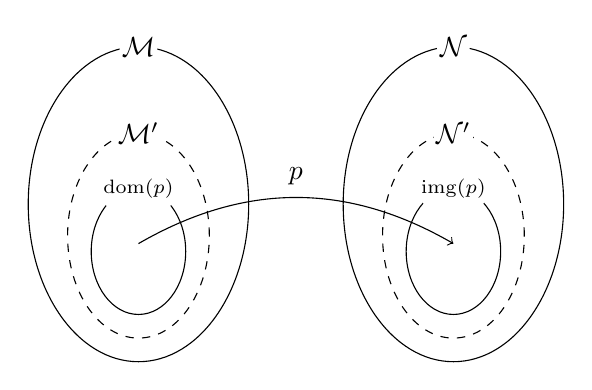
\begin{tikzpicture}
      \draw (-2,0) circle [x radius=1.4cm, y radius=2cm];
      \draw [dashed] (-2,-0.4) circle [x radius=0.9cm, y radius=1.3cm];
      \draw (-2,-0.6) circle [x radius=0.6cm, y radius=0.8cm];
      \draw (2,0) circle [x radius=1.4cm, y radius=2cm];
      \draw [dashed] (2,-0.4) circle [x radius=0.9cm, y radius=1.3cm];
      \draw (2,-0.6) circle [x radius=0.6cm, y radius=0.8cm];
      \node [fill=white, circle, inner sep=0] at (-2,2) {$\mathcal{M}$};
      \node [fill=white, circle, inner sep=0] at (-2,0.9) {$\mathcal{M}'$};
      \node [fill=white, circle, inner sep=0] at (-2,0.2) {$\scriptstyle\dom(p)$};
      \node [fill=white, circle, inner sep=0] at (2,2) {$\mathcal{N}$};
      \node [fill=white, circle, inner sep=0] at (2,0.9) {$\mathcal{N}'$};
      \node [fill=white, circle, inner sep=0] at (2,0.2) {$\scriptstyle\img(p)$};
      \draw [->] (-2,-0.5) to[bend left] (2,-0.5) node [pos=.5, label=above:$p$] {};
    \end{tikzpicture}
  \end{center}
  % picture
  Now $p$ is a \hyperlink{def:pe}{finite partial embedding} between countable models, so $p$ extends to an \hyperlink{def:iso}{isomorphism} $\pi: \mathcal{M}' \to \mathcal{N}'$ by \cref{thm:4.4}.
  In particular, $\pi$ is an \hyperlink{def:elmap}{elementary map} between $\mathcal{M}$ and $\mathcal{N}$.
\end{proof}
\begin{ncor}\label{cor:4.13}
  $\hyperlink{def:elsubs}{(\mathbb{Q}, <) \preccurlyeq (\mathbb{R}, <)}$.
\end{ncor}
\begin{proof}
  Use \cref{prop:4.12} with $\operatorname{id}: \mathbb{Q} \to \mathbb{R}$.
\end{proof}
\subsection{Random graph}
\begin{ndef}[Random graph]\label{def:4.14}
  Let $L_{\text{gph}} = \{R\}$, a binary relation symbol.
  An $L_{\text{gph}}$-\hyperlink{def:str}{structure} is a \named{graph} if
  \begin{enumerate}[label=(\roman*)]
    \item $\forall x \; \lnot R(x,x)$
    \item $\forall xy \; (R(x,y) \leftrightarrow R(y,x))$
  \end{enumerate}

  \hypertarget{def:rgraph}An $L_{\text{gph}}$-\hyperlink{def:str}{structure} is a \named{random graph} if it is a graph such that, for all $n \in \omega$, axiom $(r_n)$ holds:
      \begin{equation*}
        \forall x_0 \dots x_n, y_0 \dots y_n \; \left(\bigwedge_{i,j=0}^n x_i \neq y_j \to \exists z \; \left(\bigwedge_{i=0}^n (z \neq x_i) \land (z \neq y_i) \land R(z,x_i) \land \lnot R(z, y_i)\right)\right)
      \end{equation*}
  \begin{enumerate}[label=(\roman*)]\setcounter{enumi}{2}
    \item $\exists xy \; (x \neq y)$.
  \end{enumerate}
\end{ndef}
Axiom $(r_n)$ effectively says that for disjoint subsets $(x_i)$ and $(y_i)$ each of size $n$, there is a (different) node $z$ connected to each $x_i$ and none of the $y_i$.
\begin{center}
  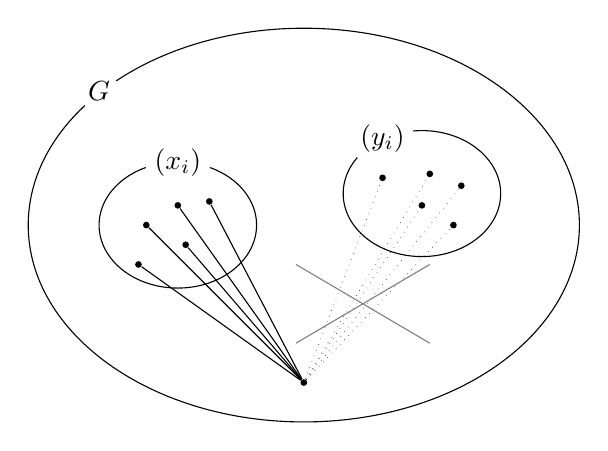
\begin{tikzpicture}
    \draw (0,0.5) circle [x radius=3.5cm, y radius=2.5cm];
    \draw (1.5,0.9) circle [x radius=1cm, y radius=0.8cm];
    \draw (-1.6,0.5) circle [x radius=1cm, y radius=0.8cm];
    \begin{scope}[every node/.style={fill=white, circle, inner sep=0.5mm}]
    \node at (-2.6,2.2) {$G$};
    \node at (-1.6, 1.3) {$(x_i)$};
    \node at (1, 1.6) {$(y_i)$};
    \end{scope}
    \begin{scope}[every node/.style={fill=black, black, circle, inner sep=0.3mm}]
      \node (z) at (0,-1.5) {};
      \node (1x) at (-1.5,0.25) {};
      \node (2x) at (-2,0.5) {};
      \node (3x) at (-1.2,0.8) {};
      \node (4x) at (-1.6,0.75) {};
      \node (5x) at (-2.1,0) {};

      \node (1y) at (1.5,0.75) {};
      \node (2y) at (2  ,1.00) {};
      \node (3y) at (1.0,1.10) {};
      \node (4y) at (1.6,1.15) {};
      \node (5y) at (1.9,0.50) {};

      \foreach \x in {1,...,5}{
        \draw (z) -- (\x x);
        \draw [dotted, very thin] (z) -- (\x y);
      }

      \draw [gray] (-0.1, 0) -- (1.6,-1);
      \draw [gray] (-0.1,-1) -- (1.6,0);
    \end{scope}
  \end{tikzpicture}
\end{center}
\begin{remark}
  A \hyperlink{def:rgraph}{random graph} is infinite.
  Given a finite subset, we can always find a vertex that is connected to every vertex in the subset (likewise for not connected).
\end{remark}
\begin{nfact}\label{fact:4.15}
  There is a \hyperlink{def:rgraph}{random graph}.
\end{nfact}
\begin{proof}
  Let the domain be $\omega$, let $i,j \in \omega$ such that $i < j$.
  Write $j$ as a sum of distinct powers of $2$.
  Then $\{i,j\}$ is an edge iff $2^i$ appears in the sum.
\end{proof}
\begin{exercise}
  Prove that $\omega$ with this definition of $R$ is a \hyperlink{def:rgraph}{random graph}.
\end{exercise}
\begin{ndef}[Graph theories, partial embedding]\label{def:4.16}\hypertarget{def:gpe}
  $T_{\text{gph}}$ consists of the axioms (i),(ii) above, and $T_{\text{rg}} = T_{\text{gph}} \cup \{(\text{iii}), (r_n) : n \in \omega\}$.
  If $\mathcal{M}$, $\mathcal{N} \models T_{\text{gph}}$, a \index{partial embedding}\textbf{partial embedding} is an injective map $p: A \subseteq M$ to $N$ such that
  \begin{equation*}
    \mathcal{M} \models R(a,b) \iff \mathcal{N} \models R(p(a), p(b))
  \end{equation*}
  for all $a,b$ in the domain.
  Just as before, if $|\dom(p)| < \omega$ then $p$ is called a \textbf{finite partial embedding}\index{partial embedding!finite}.
\end{ndef}
\begin{nlemma}[Extension lemma for random graphs]\label{lem:4.17}
  \index{Extension lemma}Let $\mathcal{M} \hyperlink{def:models}{\models} \hyperlink{def:gpe}{T_{\text{gph}}}$, $\mathcal{N} \models \hyperlink{def:gpe}{T_{\text{rg}}}$, let $p: A \subseteq M \to N$ be a \hyperlink{def:gpe}{finite partial embedding}, and let $c \in M$.
  Then there is a partial embedding $\hat{p}: \hat{A} \subseteq M \to N$ such that, $c \in \dom(\hat{p})$, and $p \subseteq \hat{p}$.
\end{nlemma}

\begin{proof}
  \marginnote{\emph{Lecture 7}}[0cm]
  Take $c \in M$, $c \notin \dom(p)$.
  \begin{center}
    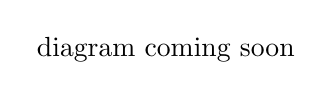
\begin{tikzpicture}
      \node {diagram coming soon};
    \end{tikzpicture}
  \end{center}
  Find $d \in N$ such that $N \models R(d, p(a)) \iff M \models R(c,a)$. %check this against notes
\end{proof}
\begin{nthm}\label{thm:4.18}
  Let $\mathcal{M},\, \mathcal{N} \hyperlink{def:models}{\models} \hyperlink{def:gpe}{T_{\text{rg}}}$ and $|\mathcal{M}| = |\mathcal{N}| = \omega$, and $p: A \subset M \to N$ a \hyperlink{def:gpe}{finite partial embedding}.
  Then $\mathcal{M} \hyperlink{def:iso}{\simeq} \mathcal{N}$, by an isomorphism that extends $p$.
\end{nthm}
\begin{proof}
  Same as proof of \cref{thm:4.4}, but with \cref{lem:4.17} instead of \cref{lem:4.3}.
\end{proof}
\begin{ncor}
  \hyperlink{def:gpe}{$T_{\text{rg}}$} is \hyperlink{def:wcat}{$\omega$-categorical} and \hyperlink{def:complete}{complete}.
  Moreover, every \hyperlink{def:gpe}{finite partial embedding} between \hyperlink{def:model}{models} of $T_{\text{rg}}$ is an \hyperlink{def:elmap}{elementary map}.
\end{ncor}
\begin{nremark}\label{rem:4.20}
  The unique (up to isomorphism) countable model of \hyperlink{def:gpe}{$T_{\text{rg}}$} is \emph{the} countable random graph, or the \named{Rado graph}.
  It is universal with respect to finite and countable graphs (i.e.\ it embeds them all).
  It is \named{ultrahomogeneous} i.e.\ every \hyperlink{def:iso}{isomorphism} between finite \hyperlink{def:subs}{substructures} extends to an automorphism of the whole graph.
\end{nremark}

\clearpage
\section{Compactness}
\begin{ndef}\label{def:5.1}
  Take an \hyperlink{def:ltheory}{$L$-theory} $T$.
  \begin{enumerate}[label=(\roman*)]
    \item \hypertarget{def:fs}$T$ is \named{finitely satisfiable} if every finite subset of \hyperlink{def:sentence}{sentences} in $T$ has a \hyperlink{def:model}{model}.
    \item \hypertarget{def:maximal}$T$ is \named{maximal} if for all $L$-sentences $\sigma$, either $\sigma \in T$ or $\lnot \sigma \in T$.
    \item \hypertarget{def:wp}$T$ has the \named{witness property} if for all $\phi(x)$ ($L$-\hyperlink{def:form}{formula} with one \hyperlink{def:free}{free} variable) there is a constant $c \in \mathscr{C}$ such that
      \begin{equation*}
        ((\exists x \; \phi(x)) \to \phi(c)) \in T.
      \end{equation*}
  \end{enumerate}
\end{ndef}
\begin{nlemma}\label{lem:5.2}
  If $T$ is \hyperlink{def:maximal}{maximal} and \hyperlink{def:fs}{finitely satisfiable} and $\varphi$ is an $L$-\hyperlink{def:sentence}{sentence}, and $\Delta \overset{\mathclap{\text{finite}}}\subseteq T$ with $\Delta \hyperlink{def:entails}{\vdash} \varphi$, then $\varphi \in T$.
\end{nlemma}
\begin{proof}
  If $\varphi \notin T$ then $\neg \varphi \in T$ (by maximality).
  But then $\Delta \cup \{\neg \varphi\}$ is a finite subset of $T$ which does not have a model.
\end{proof}
\begin{nlemma}\label{lem:5.3}
  Let $T$ be a \hyperlink{def:maximal}{maximal}, \hyperlink{def:fs}{finitely satisfiable} theory with the \hyperlink{def:wp}{witness property}.
  Then $T$ has a \hyperlink{def:model}{model}.
  Moreover, if $\lambda$ is a cardinal and $|\hyperlink{def:lang}{\mathscr{C}}| \leq \lambda$, then $T$ has a model of size at most $\lambda$.
\end{nlemma}
\begin{proof}
  Let $c,d \in \hyperlink{def:lang}{\mathscr{C}}$, define $c \sim d$ iff $c = d \in T$.

  \textbf{Claim:} $\sim$ is an equivalence relation. \textbf{Proof:} For transitivity, let $c \sim d$ and $d \sim e$.
  Then $c = d \in T$ and $d = e \in T$, so $c = e \in T$ (by \cref{lem:5.2}), and so $c \sim e$. Reflexivity follows from \hyperlink{def:maximal}{maximality}, and symmetry is immediate. $\blacksquare$

  \hypertarget{def:cstar}We denote $[c] \in \mathscr{C} / \sim$ by $c^*$.
  Now, define a \hyperlink{def:str}{structure} $\mathcal{M}$ whose domain is $\mathscr{C} / \sim\ = M$.
  Clearly, $|M| \leq \lambda$ if $|\mathscr{C}| \leq \lambda$.
  We must define \hyperlink{def:str}{interpretations} in $\mathcal{M}$ for symbols of $L$.
  \begin{itemize}
    \item If $c \in \mathscr{C}$, then $c^\mathcal{M} = c^*$.
    \item If $R \in \mathscr{R}$, define
      \begin{equation*}
        R^\mathcal{M} \coloneqq \set{(c_1^*, \dotsc, c_{n_R}^*) | R(c_1, \dotsc, c_n) \in T}.
      \end{equation*}
      \textbf{Claim:} $R^\mathcal{M}$ is well defined.
      \textbf{Proof:} Suppose $\bar{c}, \bar{d} \in \mathscr{C}^{n_R}$ and suppose $c_i \sim d_i$.
      That is, $c_i = d_i \in T$ for $i=1, \dotsc, n_R$ so by \cref{lem:5.2}
      \begin{equation*}
        R(\bar{c}) \in T \iff R(\bar{d}) \in T. \tag*{$\blacksquare$}
      \end{equation*}
    \item If $f \in \mathscr{F}$, and $\bar{c} \in \mathscr{C}^{n_R}$, then $f \bar{c} = d \in T$ for some $d \in \mathscr{C}$.
      (This is because $\exists x \; (f(\bar{c}) = x) \in T$ so apply \hyperlink{def:wp}{witness property}.)

      Then define $f^\mathcal{M}(\bar{c}^*) = d^*$.
      Exercise: Check $f^\mathcal{M}(\bar{c}^*)$ is well-defined!
  \end{itemize}

  \textbf{Claim:} if $t(x_1, \dotsc, x_n)$ is an \hyperlink{def:lterm}{$L$-term} and $c_1, \dotsc, c_n, d \in \mathscr{C}$, then
  \begin{equation*}
    t(c_1, \dotsc, c_n) = d \in T \iff t^\mathcal{M}(c_1^*, \dotsc, c_n^*) = d^*.
  \end{equation*}
  \textbf{Proof:}
  \begin{itemize}
    \item [$(\Rightarrow)$] by induction on the complexity of $t$.
    \item [$(\Leftarrow)$] Assume $t^\mathcal{M}(c_1^*, \dotsc, c_n^*) = d^*$.
    Then
    \begin{equation*}t(c_1, \dotsc, c_n) = e \in T\end{equation*}
    for some constant $e$ by \hyperlink{def:wp}{witness property} and \cref{lem:5.2}.
    Use ($\Rightarrow$) to get that $t^\mathcal{M}(c_1^*, \dotsc, c_n^*) = e^*$.
    But then $d^* = e^*$, i.e.\ $d = e \in T$.
    Then $t(c_1, \dotsc, c_n) = d \in T$. $\blacksquare$
  \end{itemize}

  \textbf{Claim:} For all $L$-formulas $\varphi(\bar{x})$, and $\bar{c} \in \mathscr{C}^{|\bar{x}|}$,
  \begin{equation*}
    \mathcal{M} \models \varphi(\bar{c}) \iff \varphi(\bar{c}) \in T.
  \end{equation*}
  \textbf{Proof:} By induction on $\varphi(\bar{x})$. (Exercise: Fill in the details).  $\blacksquare$
  This shows $\mathcal{M} \models T$.
\end{proof}
\begin{nlemma}\label{lem:5.4}
  \marginnote{\emph{Lecture 8}}[0cm]
  Let $T$ be a \hyperlink{def:fs}{finitely satisfiable} \hyperlink{def:ltheory}{$L$-theory}.
  Then there are $L^* \supseteq L$ and a finitely satisfiable $L^*$-theory $T^* \supseteq T$ such that
  \begin{enumerate}[label=(\roman*)]
    \item $|L^*| = |L| + \omega$.
    \item any $L^*$-theory extending $T^*$ has the \hyperlink{def:wp}{witness property}.
  \end{enumerate}
\end{nlemma}
\begin{proof}
  We define $\langle L_i : i < \omega \rangle$ a \hyperlink{def:chain}{chain} of \hyperlink{def:lang}{languages} containing $L$ and such that $|L_i| = |L| + \omega$, and $\langle T_i : i < \omega \rangle$ of \hyperlink{def:fs}{finitely satisfiable} \hyperlink{def:ltheory}{theories} such that $\forall i, T_i$ is an $L_i$-theory and $T_i \supseteq T$.

  Set $L_0 = L$ and $T_0 = T$. At stage $i+1$, $L_i$ and $T_i$ are given.
  List all \hyperlink{def:form}{$L_i$-formulas} $\varphi(x)$ (one \hyperlink{def:free}{free} variable) and let
  \begin{equation*}L_{i+1} = L_i \cup \set{c_\varphi | \varphi(x) \text{ an } L_i \text{ formula}}.\end{equation*}
  For all $\varphi(x)$, an $L_i$ formula in one free variable, let $\Phi_\varphi$ be the $L_{i+1}$-sentence
  \begin{equation*}
    \exists x \; \varphi(x) \to \varphi(c_\varphi).
  \end{equation*}
  Then let
  \begin{equation*}T_{i+1} = T_i \cup \set{\Phi_\varphi | \varphi(x)\text{ is an }L_i\text{ formula}}.\end{equation*}

  \textbf{Claim}: $T_{i+1}$ is \hyperlink{def:fs}{finitely satisfiable}.

  \textbf{Proof}: Let $\Delta \subseteq T_{i+1}$ be finite.
  Then
  \begin{equation*}\Delta = \Delta_0 \cup \{\Phi_{\varphi_1}, \dotsc, \Phi_{\varphi_n}\}\end{equation*}
  where $\Delta_0 \subseteq T_i$.
  Let $\mathcal{M} \models \Delta_0$ ($\mathcal{M}$ is an \hyperlink{def:str}{$L_i$ structure}; it exists because $T_i$ is \hyperlink{def:fs}{finitely satisfiable}).

  We define an $L_{i+1}$-structure $\mathcal{M}'$ with domain $M$.
  Define the \hyperlink{def:str}{interpretation} of new constants as follows:
  if $\mathcal{M} \models \exists x \; \varphi(x)$, then let $a$ be such that $\mathcal{M} \models \varphi(a)$, and set $c_\varphi^{\mathcal{M}'} \coloneqq a$.
  Otherwise, $c_\varphi^{\mathcal{M}'}$ is arbitrary. Then $\mathcal{M}' \models \Delta$. $\blacksquare$

  Let
  \begin{equation*}L^* = \bigcup_{i < \omega} L_i, \qquad T^* = \bigcup_{i < \omega} T_i.\end{equation*}
  By construction, any extension of $T^*$ has the \hyperlink{def:wp}{witness property} (check this!) and $T^*$ is finitely satisfiable.
  (If $\Delta \overset{\mathclap{\text{finite}}}\subseteq T^*$ then $\Delta \subseteq T_i$ for some $i$).
\end{proof}
\begin{nlemma}\label{lem:5.5}
  If $T$ is \hyperlink{def:fs}{finitely satisfiable}, there exists a \hyperlink{def:maximal}{maximal} finitely satisfiable $T' \supseteq T$.
\end{nlemma}
\begin{proof}
  Let
  \begin{equation*}
    I \coloneqq \set{S | S\text{ is a \hyperlink{def:fs}{finitely satisfiable} \hyperlink{def:ltheory}{$L$-theory} such that }T \subseteq S}.
  \end{equation*}
  $I$ is partially ordered by inclusion, and non-empty.

  If $\langle C_i : i < \lambda \rangle$ is a \hyperlink{def:chain}{chain} in $I$, then $\bigcup_{i < \lambda} C_i$ is an upper bound for the chain - it is finitely satisfiable.
  Then by Zorn's lemma, $I$ has a maximal element (with respect to $\subseteq$).

  \textbf{Claim:} the maximal element $T'$ of $I$ is the required extension of $T$ (check that for all \hyperlink{def:sentence}{$L$-sentences} $\sigma$, $\sigma \in T'$ or $\lnot \sigma \in T'$).
\end{proof}
\begin{nthm}[Compactness]\label{thm:5.6}
  \index{compactness}If $T$ is a \hyperlink{def:fs}{finitely satisfiable} \hyperlink{def:ltheory}{$L$-theory} and $\lambda \geq |L| + \omega$, then there is $\mathcal{M} \hyperlink{def:models}{\models} T$ such that $|\mathcal{M}| \leq \lambda$.
\end{nthm}
\begin{proof}[Proof sketch]
  Extend $T$ to $T^*$, an $L^*$-theory that is \hyperlink{def:fs}{finitely satisfiable} and such that any $S \supseteq T^*$ has the \hyperlink{def:wp}{witness property} (by \cref{lem:5.4}).

  By \cref{lem:5.5}, there is $T' \supseteq T^*$, which is \hyperlink{def:maximal}{maximal} and \hyperlink{def:fs}{finitely satisfiable}.
  Then $T'$ has the \hyperlink{def:wp}{witness property}.
  Then by \cref{lem:5.3} there is $\mathcal{M} \models T'$ with $|\mathcal{M}| \leq \lambda$, and $\mathcal{M} \models T$.
\end{proof}
\begin{ndef}[Type]\label{def:5.7}\hypertarget{def:type}
  Let $L$ be a \hyperlink{def:lang}{language}.
  \begin{itemize}
    \item An $L$-\named{type} $p(\bar{x})$ is a set of \hyperlink{def:form}{$L$-formulas} whose \hyperlink{def:free}{free} variables are in $\bar{x}$ (and $\bar{x} = \langle x_i : i < \lambda \rangle$).

    \item An $L$-type is \named{satisfiable}\index{type!satisfiable} if there is an \hyperlink{def:str}{$L$-structure} $\mathcal{M}$ and an assignment $\bar{a} \in \mathcal{M}^{|\bar{x}|}$ to $\bar{x}$ such that $\mathcal{M} \models \varphi(\bar{a})$ for all $\varphi(\bar{x}) \in p(\bar{x})$ (we also say $p(\bar{x})$ \named{consistent}, and that $\bar{a}$ \named{realizes} $p(\bar{x})$ in $\mathcal{M}$).
      We write $\mathcal{M} \models p(\bar{a})$ or $\mathcal{M},\bar{a} \models p(\bar{x})$.
    We also say that $p(\bar{x})$ is \textbf{satisfied} in $\mathcal{M}$.

    \item A type $p(\bar{x})$ is \named{finitely satisfiable} if every finite subset of $p(x)$ is satisfiable (we may say $p(\bar{x})$ is \textbf{finitely consistent}).
  \end{itemize}
\end{ndef}
\begin{remark}
  An $L$-\hyperlink{def:type}{type} may be \hyperlink{def:type}{finitely satisfiable} in $\mathcal{M}$ (i.e. every finite subset is \hyperlink{def:type}{satisfiable} in $\mathcal{M}$) but not satisfiable in $\mathcal{M}$.
\end{remark}
\begin{eg}
  Take $\mathcal{M} = (\mathbb{N}, <)$. Let $\phi_n(x)$ say `there are at least $n$ elements less than $x$'.
  \begin{equation*}
    p(x) \coloneqq \set{\phi_n(x) | n < \omega}
  \end{equation*}
  Is $p(x)$ \hyperlink{def:type}{finitely satisfiable} in $\mathcal{M}$? Yes. But $p(x)$ is not \hyperlink{def:type}{satisfiable} in $\mathcal{M}$.
\end{eg}
\begin{nthm}[Compactness theorem for types]\label{thm:5.8}
  Every \hyperlink{def:type}{finitely satisfiable} \hyperlink{def:type}{$L$-type} $p(\bar{x})$ is \hyperlink{def:type}{satisfiable}.
\end{nthm}
\begin{proof}
  Let $\bar{x} = \langle x_i : i < \lambda \rangle$, let $\langle c_i : i < \lambda \rangle$ be new constants (not in $L$).
  Expand $L$ to $L' = L \cup \{c_i : i < \lambda\}$.
  Then $p(\bar{c})$ is a \hyperlink{def:fs}{finitely satisfiable} \hyperlink{def:ltheory}{$L'$-theory} and \cref{thm:5.6} applied to $p(\bar{c})$ gives an $L'$-structure $\mathcal{M}'$ such that $\mathcal{M}' \models p(\bar{c})$.
  But $\mathcal{M}'$ reduces to an $L$ structure $\mathcal{M}$, so $\mathcal{M}, \bar{c}^{\mathcal{M}'} \models p(\bar{x})$.
\end{proof}
\begin{nlemma}\label{lem:5.9}
  \marginnote{\emph{Lecture 9}}
  Let $\mathcal{M}$ be a \hyperlink{def:str}{structure}, let $\bar{a} = \langle a_i : i < \lambda \rangle$ an enumeration of $\mathcal{M}$.
  Let
  \begin{equation*}q(\bar{x}) = \set{\varphi(\bar{x}) | \mathcal{M} \models \varphi(\bar{a})},\end{equation*}
  where $|\bar{x}| < \lambda$.
  Then $q(\bar{x})$ is \hyperlink{def:type}{satisfiable} in $\mathcal{N}$ iff there is $\beta: \mathcal{M} \to \mathcal{N}$ that is an \hyperlink{def:el}{elementary embedding}.
\end{nlemma}
\begin{proof}\leavevmode
  \begin{itemize}
    \item[($\Rightarrow$)] If $q(\bar{x})$ is \hyperlink{def:type}{satisfiable} in $\mathcal{N}$, there is $\bar{b} \in N^{|\bar{x}|}$ such that
  \begin{equation*}
    \mathcal{N} \models \varphi(\bar{b}) \quad \forall \varphi(\bar{x}) \in q(\bar{x}).
  \end{equation*}

  Then $\beta: a_i \mapsto b_i$ for $i < \lambda$ is an \hyperlink{def:el}{elementary embedding}.
  ($\beta$ preserves, for example, \hyperlink{def:atomform}{atomic formulas} of the form $f(a_{i_1}, \dotsc, a_{i_n}) = a_{i_{n+1}}$).
  More generally, for any $\varphi(\bar{x})$ an \hyperlink{def:form}{$L$-formula},
  \begin{equation*}
    \mathcal{M} \models \varphi(\bar{a}) \iff \mathcal{N} \models \varphi(\bar{b})
  \end{equation*}
  but $\beta(\bar{a}) = \bar{b}$ so we have \hyperlink{def:el}{elementarity}.

  \item[($\Leftarrow$)] If $\beta: \mathcal{M} \to \mathcal{N}$ is elementary, then $\beta(\bar{a})$ satisfies $q(\bar{x})$ in $\mathcal{N}$. \qedhere
  \end{itemize}
\end{proof}
This lemma is sometimes also called the Diagram Lemma, and stated as: Suppose $\Th(\mathcal{M}_M)$ is a theory in $L(M)$.
Then if $\mathcal{N} \hyperlink{def:models}{\models} \Th(\mathcal{M}_M)$, then $\mathcal{M}$ \hyperlink{def:el}{embeds elementarily} in $\mathcal{N}$.
\begin{nremark}\label{rem:5.10}
  We can consider types in $\hyperlink{def:la}{L(A)}$, where $A \subseteq M$.
  In particular, we can have $M = A$.

  \hypertarget{def:typeparam}Types of this kind are said to have \textbf{parameters in $A$} (or to be over $A$).
  If $p(\bar{x})$ is a type over $M$, then there is $\bar{a}$, an enumeration of $M$, and a type $p'(\bar{x}, \bar{z})$ in $L$ where the $\bar{z}$ are new constants, $|\bar{z}| = |\bar{a}|$, and $p(\bar{x}) = p'(\bar{x}, \bar{a})$.
\end{nremark}
\begin{nthm}\label{thm:5.11}
  If $\mathcal{M}$ is a \hyperlink{def:str}{structure}, and $p(\bar{x})$ is a \hyperlink{def:type}{type} in $L(M)$ that is \hyperlink{def:type}{finitely satisfiable} in $\mathcal{M}$, then $p(\bar{x})$ is \hyperlink{def:type}{satisfiable} in some $\mathcal{N}$ such that $\mathcal{M} \hyperlink{def:elsubs}{\preccurlyeq} \mathcal{N}$.
\end{nthm}
\begin{eg}
  Take $\mathcal{M} = (\mathbb{Q}, <)$, and let $\langle a_i : i < \omega \rangle$ a sequence in $\mathbb{Q}$ that converges to $\sqrt{2}$ from below, and let $\langle b_i : i < \omega \rangle \subseteq \mathbb{Q}$ tend to $\sqrt{2}$ from above.
  Set $\phi_n(x) \coloneqq a_n < x < b_n$. Then let $p(x) = \set{\phi_n(x) | n < \omega}$.
  Then $p(x)$ is an $L(\mathbb{Q})$-\hyperlink{def:type}{type} which is \hyperlink{def:type}{finitely satisfiable} in $\mathbb{Q}$.
  But $p(x)$ is not \hyperlink{def:type}{satisfiable} in $\mathcal{M}$.
  It is, however, satisfiable in $(\mathbb{R}, <) \succcurlyeq (\mathbb{Q}, <)$.
\end{eg}
\begin{proof}[Proof of \cref{thm:5.11}]
  Let $\langle a_i : i < \lambda \rangle$ enumerate $\mathcal{M}$, let
  \begin{equation*}q(\bar{z}) \coloneqq \set{\varphi(\bar{z}) | \mathcal{M} \models \varphi(\bar{a})}\end{equation*}
  where $|\bar{z}| = \lambda$ and the $z_i$ are new variables (so not among the $\bar{x}$).
  Write $p(\bar{x})$ as $p'(\bar{x}, \bar{a})$ for some $p'(\bar{x}, \bar{z})$ (an $L$-\hyperlink{def:type}{type}).

  \textbf{Claim}: $p'(\bar{x},\bar{z}) \cup q(\bar{z})$ is \hyperlink{def:type}{finitely satisfiable} in $\mathcal{M}$.

  \textbf{Proof:} $p'(\bar{x},\bar{a})$ is finitely satisfiable by hypothesis and $q(\bar{z})$ is \hyperlink{def:type}{realized} by $\bar{a}$.

  Then, by \nameref{thm:5.8}, $p'(\bar{x}, \bar{z}) \cup q(\bar{z})$ is satisfiable.
  That is, there is $\mathcal{N}$ and $\bar{b} \in \mathcal{N}^{|\bar{z}|}$ and $\bar{c} \in \mathcal{N}^{|\bar{x}|}$ such that
  \begin{equation*}
    \mathcal{N} \models p'(\bar{c}, \bar{b}) \cup q(\bar{b}).
  \end{equation*}
  In particular, $\mathcal{N} \models q(\bar{b})$, then by \cref{lem:5.9}, $\beta: a_i \mapsto b_i$ is an \hyperlink{def:el}{elementary embedding}.
\end{proof}
\begin{nthm}[Upward L\"owenheim-Skolem]\label{thm:5.12}
  Let $\mathcal{M}$ be such that $|\mathcal{M}| \geq \omega$.
  Then for any $\lambda \geq |\mathcal{M}| + |L|$, there is $\mathcal{N}$ such that \hyperlink{def:elsubs}{$\mathcal{M} \preccurlyeq \mathcal{N}$}, and $|\mathcal{N}| = \lambda$.
\end{nthm}
\begin{proof}
  Let $\bar{x} = \langle x_i : i < \lambda \rangle$ a tuple of distinct variables.
  Let
  \begin{equation*}
    p(\bar{x}) = \set{x_i \neq x_j | i < j < \lambda}.
  \end{equation*}
  Then $p(\bar{x})$ is \hyperlink{def:type}{finitely consistent} in $\mathcal{M}$.
  By \cref{thm:5.11}, $p(\bar{x})$ is \hyperlink{def:type}{realized} in some $\mathcal{M} \preccurlyeq \mathcal{N}$, and $|\mathcal{N}| \geq \lambda$.
  By \nameref{thm:3.11DLS}, we may assume $|\mathcal{N}| = \lambda$.
\end{proof}

\clearpage
\section{Saturation}
\begin{ndef}[Saturated]\label{def:6.1}\hypertarget{def:sat}
  Let $\lambda$ be an infinite cardinal, let $|\mathcal{M}| \geq \omega$.
  Then $\mathcal{M}$ is \textbf{$\lambda$-saturated} if $\mathcal{M}$ \hyperlink{def:type}{realizes} every \hyperlink{def:type}{type} $p(x)$ with one \hyperlink{def:free}{free variable} such that
  \begin{enumerate}[label=(\roman*)]
    \item $p(x)$ has \hyperlink{def:typeparam}{parameters} in $A \subseteq M$ and $|A| < \lambda$.
    \item $p(x)$ is \hyperlink{def:type}{finitely consistent} in $\mathcal{M}$.
  \end{enumerate}
  $\mathcal{M}$ is \named{saturated} if it is $|\mathcal{M}|$-saturated.
\end{ndef}

Can $\mathcal{M}$ be \hyperlink{def:sat}{$\lambda$-saturated} if $\lambda > |\mathcal{M}|$? If so, $\mathcal{M}$ would satisfy \hyperlink{def:type}{finitely satisfiable types} in $L(M)$.
For example,
\begin{equation*}
    p(x) = \set{x \neq a_i | i < |\mathcal{M}|}
\end{equation*}
where $\langle a_i : i < |\mathcal{M}| \rangle$ enumerates $\mathcal{M}$. $p(x)$ is finitely satisfiable, but not satisfied in $\mathcal{M}$.

\begin{ndef}[Type of tuple]\label{def:6.2}
  \marginnote{\emph{Lecture 10}}
  \hypertarget{def:tp}Let $\mathcal{M}$ be an \hyperlink{def:str}{$L$-structure}, $A \subseteq M$, $\bar{b}$ a tuple in $M$ (possibly infinite).
  The \textbf{type of $\bar{b}$ over $A$} is the following $L(A)$-\hyperlink{def:type}{type}:
  \begin{equation*}
    \tp_\mathcal{M}(\bar{b}/A) \coloneqq \set{\varphi(\bar{x}) \in L(A) | \mathcal{M} \models \varphi(\bar{b})}.
  \end{equation*}
  The subscript $\mathcal{M}$ is often omitted if clear from context.
\end{ndef}
\begin{nremark}\label{rem:6.3}\leavevmode
  \begin{enumerate}[label=(\roman*)]
    \item $\hyperlink{def:tp}{\tp_{\mathcal{M}}(\bar{b}/A)}$ is \hyperlink{def:complete}{complete}, i.e.\ for every $L(A)$ \hyperlink{def:form}{formula} $\phi(\bar{x})$, either $\phi(\bar{x}) \in \tp(\bar{b}/A)$ or $\lnot \phi(x) \in \tp(\bar{b}/A)$.
    \item If $\hyperlink{def:elsubs}{\mathcal{M} \preccurlyeq \mathcal{N}}$, then for $A \subseteq M$, $\bar{b}$ a tuple:
      \begin{equation*}
        \tp_\mathcal{M}(\bar{b}/A)= \tp_\mathcal{N}(\bar{b}/A).
      \end{equation*}
  \end{enumerate}
\end{nremark}
\begin{nfact}\label{fact:6.4}\leavevmode
  \begin{enumerate}[label=(\roman*)]
    \item If $f: A \subseteq \mathcal{M} \to \mathcal{N}$ is a (partial) \hyperlink{def:elmap}{elementary map}, then in particular $f$ preserves \hyperlink{def:sentence}{$L$-sentences}, so $\mathcal{M} \hyperlink{def:eleq}{\equiv} \mathcal{N}$.
    \item If $\mathcal{M} \equiv \mathcal{N}$, then $\emptyset$, the empty map, is an \hyperlink{def:el}{elementary map}, as it preserves sentences.
    \item If $f: A \subseteq \mathcal{M} \to \mathcal{N}$ is elementary, and $\bar{a}$ is an enumeration of $A = \dom(f)$, then
      \begin{equation*}
        \tp(\bar{a}/\emptyset) = \tp(f(\bar{a})/\emptyset).
      \end{equation*}
      More generally, if $f: \mathcal{M} \to \mathcal{N}$ is (partial) elementary and there is $A \subseteq M \cap N$ such that $A \subseteq \dom f$, $f|_A = \operatorname{id}$, then for every $\bar{b}$, a tuple in $\dom(f)$,
      \begin{equation*}
        \tp_\mathcal{M}(\bar{b}/A) = \tp_{\mathcal{N}}(f(\bar{b})/A).
      \end{equation*}
      %\begin{center}
      %  \begin{tikzpicture}
      %  \end{tikzpicture}
      %\end{center}
    \item Let $\bar{a}$ enumerate $A \subseteq M$, $A = \dom(f)$ where $f: \mathcal{M} \to \mathcal{N}$ is elementary.
      Let $p(\bar{x},\bar{a})$ be a \hyperlink{def:type}{type} in $L(A)$ that is \hyperlink{def:type}{finitely satisfiable} in $\mathcal{M}$.
      Then $p(\bar{x},f(\bar{a}))$ is finitely satisfiable in $\mathcal{N}$:

      Let
      \begin{equation*}\{\varphi_1(\bar{x},\bar{a}), \dotsc, \varphi_n(\bar{x},\bar{a})\} \subseteq p(\bar{x},\bar{a}).\end{equation*}
      By finite satisfiability of $p(\bar{x},\bar{a})$,
    \begin{equation*}\mathcal{M} \models \exists \bar{x} \; \bigwedge_{i=1}^n \varphi_i(\bar{x},\bar{a}).\end{equation*}
      Then
      \begin{equation*}\mathcal{N} \models \exists x \; \bigwedge_{i=1}^m \varphi_i(\bar{x},f(\bar{a}))\end{equation*}
      by elementarity of $f$.
      (Does $p(\bar{x},\bar{a})$ satisfiable in $\mathcal{M}$ imply $p(\bar{x},f(\bar{a}))$ satisfiable in $\mathcal{N}$? No.)
  \end{enumerate}
\end{nfact}
\begin{nthm}\label{thm:6.5}
  Let $\mathcal{N}$ be such that $|\mathcal{N}| \geq \lambda \geq |L|+\omega$. The following are equivalent:
  \begin{enumerate}[label=(\roman*)]
    \item $\mathcal{N}$ is \hyperlink{def:sat}{$\lambda$-saturated}.
    \item if $\mathcal{M} \hyperlink{def:eleq}{\equiv} \mathcal{N}$, $b \in M$ and $f: \mathcal{M} \to \mathcal{N}$ \hyperlink{def:elmap}{partial elementary map} such that $|f| < \lambda$, then there is a partial elementary $\hat{f} \supseteq f$ and such that $b \in \dom(\hat{f})$.
    \item If $p(\bar{z})$ is an \hyperlink{def:typeparam}{$L(A)$-type} where $|\bar{z}| \leq \lambda$ and $|A| < \lambda$ and $p(\bar{z})$ is \hyperlink{def:type}{finitely satisfiable} in $\mathcal{N}$, then $p(\bar{z})$ is \hyperlink{def:type}{satisfiable} in $\mathcal{N}$.
  \end{enumerate}
\end{nthm}
\begin{proof}
  (i) $\Rightarrow$ (ii). Let $f: \mathcal{M} \to \mathcal{N}$ be as in (ii), let $b \in M$.
  Let $\bar{a}$ be an enumeration of $\dom(f)$, so $|\bar{a}| < \lambda$. Let
  \begin{equation*}
    p(x / \bar{a}) \coloneqq \hyperlink{def:tp}{\tp_\mathcal{M}}(b/\bar{a}).
  \end{equation*}
  \begin{center}
    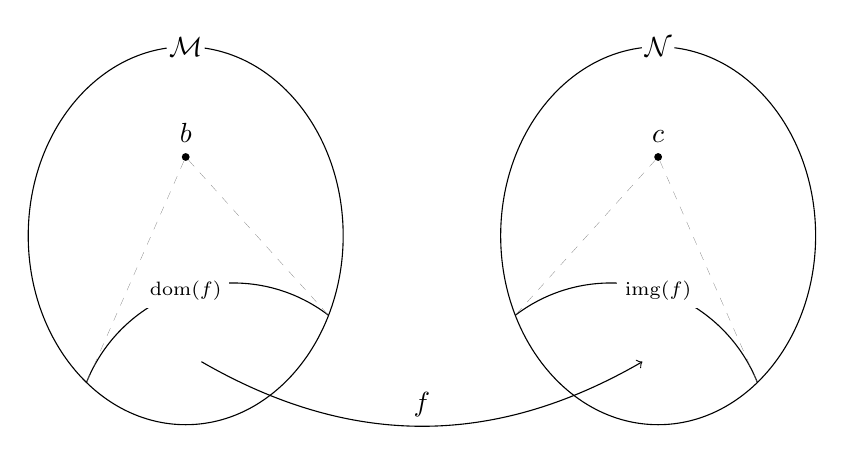
\begin{tikzpicture}[scale=2]
      \draw [name path=M] (-1.5,0) circle [x radius=1cm, y radius=1.2cm];
      \node [fill=white, circle, inner sep=0] at (-1.5,1.2) {$\mathcal{M}$};
      \draw [name path=N] (1.5,0) circle [x radius=1cm, y radius=1.2cm];
      \node [fill=white, circle, inner sep=0] at (1.5,1.2) {$\mathcal{N}$};
      \draw [->] (-1.4, -0.8) to[bend right=30] node[midway, above] {$f$} (1.4,-0.8);
      \begin{scope}
        \clip (-1.5,0) circle [x radius=1cm, y radius=1.2cm];
        \draw [name path=D] (-1.2,-1.3) circle [radius=1cm];
        \node [fill=white, rectangle, inner sep=1mm] at (-1.5,-0.35) {$\scriptstyle\dom(f)$};
        \node [fill=black, inner sep=1pt, circle, label=above:$b$] (b) at (-1.5,0.5) {};
        \path [name intersections={of=D and M}];
        \draw [dashed, gray, ultra thin] (b) -- (intersection-1);
        \draw [dashed, gray, ultra thin] (b) -- (intersection-2);
      \end{scope}
      \begin{scope}
        \clip (1.5,0) circle [x radius=1cm, y radius=1.2cm];
        \draw [name path=I] (1.2,-1.3) circle [radius=1cm];
        \node [fill=white, rectangle, inner sep=1mm] at (1.5,-0.35) {$\scriptstyle\img(f)$};
        \node [fill=black, inner sep=1pt, circle, label=above:$c$] (c) at (1.5,0.5) {};
        \path [name intersections={of=I and N}];
        \draw [dashed, gray, ultra thin] (c) -- (intersection-1);
        \draw [dashed, gray, ultra thin] (c) -- (intersection-2);
      \end{scope}
    \end{tikzpicture}
  \end{center}
  Then $p(x/\bar{a})$ is \hyperlink{def:type}{finitely satisfiable} in $\mathcal{M}$, hence $\tp(x/f(\bar{a}))$ is finitely satisfiable in $\mathcal{N}$ (by \cref{fact:6.4}(iv)).
  Since $|f(\bar{a})| < \lambda$ and $\mathcal{N}$ is \hyperlink{def:sat}{$\lambda$-saturated}, $\tp(x/f(\bar{a}))$ is \hyperlink{def:type}{realized} in $\mathcal{N}$ by some $c$.
  Then $f \cup \{\langle b,c \rangle\}$ is the required extension of $f$:
  \begin{equation*}
    \mathcal{M} \models \phi(b,\bar{a}) \iff \mathcal{N} \models \phi(c, f(\bar{a}))
  \end{equation*}

\marginnote{\emph{Lecture 11}}
  (ii) $\Rightarrow$ (iii). %Let $p(\bar{z})$ be as in (iii), $p(\bar{z})$ is finitely satisfiable in $\mathcal{N}$. Then by \cref{thm:5.11}, $p(\bar{z})$ is realized in some $\mathcal{M}' \succcurlyeq \mathcal{N}$, by some tuple $\bar{b}$ (where $|\bar{b}| = |\bar{z}|$).
  Let $p(\bar{z})$ be as in (iii). There is $\mathcal{M}$ such that $\mathcal{N} \preccurlyeq \mathcal{M}$ and $\mathcal{M} \models p(\bar{b})$.
  The identity map $\operatorname{id}_A: \mathcal{M} \to \mathcal{N}$ is \hyperlink{def:elmap}{partial elementary}.
  Idea: build $\langle f_i : i < |\bar{b}| \rangle$ of partial elementary maps extending $\operatorname{id}_A$.
  Then $\bigcup_i f_i$ is partial elementary, and $\bar{b} \in \dom \bigcup_{i < |\bar{a}|} f_i$.

  Set $f_0 = \operatorname{id}_A$, at stage $i+1$ use $(ii)$ to put $b_i$ in $\dom(f_{i+1})$.
  At limit stages, $\mu < \lambda$, let $f_{\mu} = \bigcup_{i < \mu} f_i$.

  (iii) $\Rightarrow$ (i) is trivial.
  % By Downward LS Theorem, there is $\mathcal{M} \preccurlyeq \mathcal{M}'$ such that $A \cup \{\bar{b}\} \subseteq M$, parameter set of the type.
\end{proof}
\begin{ncor}\label{cor:6.6}
  If $\mathcal{M}$ and $\mathcal{N}$ are \hyperlink{def:sat}{saturated} and $\mathcal{M} \hyperlink{def:eleq}{\equiv} \mathcal{N}$ and $|\mathcal{M}| = |\mathcal{N}|$ then any \hyperlink{def:elmap}{elementary} $f: \mathcal{M} \to \mathcal{N}$ extends to an \hyperlink{def:iso}{isomorphism} (in particular \hyperlink{def:iso}{$\mathcal{M} \simeq \mathcal{N}$}).
\end{ncor}
\begin{proof}
  Use \cref{thm:6.5}(ii) to extend $f: \mathcal{M} \to \mathcal{N}$ to an \hyperlink{def:iso}{isomorphism} by back-and-forth (take unions at limit stages).
\end{proof}
\begin{ncor}\label{cor:6.7}
  Models of of $T_{\text{dlo}}$ and $T_{\text{rg}}$ are \hyperlink{def:sat}{$\omega$-saturated}.
\end{ncor}
\begin{proof}
  By \cref{thm:6.5} and \cref{lem:4.3} for $T_{\text{dlo}}$ and \cref{lem:4.17} for $T_{\text{rg}}$.
\end{proof}

So $(\mathbb{Q}, <)$ is \hyperlink{def:sat}{$\omega$-saturated}.
Is $(\mathbb{R}, <)$ $\omega_1$ saturated? No. It does not realize
\begin{equation*}p(x) \coloneqq \set{x > q | q \in \mathbb{Q}}.\end{equation*}

\begin{ndef}[Automorphism]\label{def:6.8}
  \hypertarget{def:aut}An isomorphism $\alpha: \mathcal{N} \to \mathcal{N}$ is called an \named{automorphism}.
  The automorphisms of $\mathcal{N}$ form a group denoted by $\Aut(\mathcal{N})$.
  If $A \subseteq N$, then
  \begin{equation*}\Aut(\mathcal{N}/A) \coloneqq \set{\alpha \in \Aut(\mathcal{M}) | \alpha|_A = \operatorname{id}}.\end{equation*}
\end{ndef}
\begin{ndef}[Universality, homogeneity]\label{def:6.9}\leavevmode
  \begin{enumerate}[label=(\roman*)]
    \item \hypertarget{def:univ}An \hyperlink{def:str}{$L$-structure} $\mathcal{N}$ is \index{universal}\textbf{$\lambda$-universal} if for every \hyperlink{def:eleq}{$\mathcal{M} \equiv \mathcal{N}$} such that $|\mathcal{M}| \leq \lambda$ there is an \hyperlink{def:el}{elementary embedding} $\beta: \mathcal{M} \to \mathcal{N}$. $\mathcal{N}$ is \textbf{universal} if it is $|\mathcal{N}|$-universal.
    \item \hypertarget{def:homogeneous}$\mathcal{N}$ is \index{homogeneous}\textbf{$\lambda$-homogeneous} if every elementary map $f: \mathcal{N} \to \mathcal{N}$ such that $|f| < \lambda$ extends to an \hyperlink{def:iso}{isomorphism} of $\mathcal{N}$.
  \end{enumerate}
\end{ndef}
% Homogeneity is sometimes called `strong homogeneity'
% Ultra homogeneity contains partial embeddings

\begin{nthm}\label{thm:6.10}
  Let $\mathcal{N}$ be such that $|\mathcal{N}| \geq \hyperlink{def:cardlang}{|L|} + \omega$. The following are equivalent
  \begin{enumerate}[label=(\roman*)]
    \item $\mathcal{N}$ is \hyperlink{def:sat}{saturated}
    \item $\mathcal{N}$ is \hyperlink{def:univ}{universal} and \hyperlink{def:homogeneous}{homogeneous}.
  \end{enumerate}
\end{nthm}
\begin{proof}
  (i) $\Rightarrow$ (ii). Assume $\mathcal{N}$ is \hyperlink{def:sat}{saturated}, and $\mathcal{M} \hyperlink{def:eleq}{\equiv} \mathcal{N}$ is such that $|\mathcal{M}| \leq |\mathcal{N}|$.
  Then let $\bar{a}$ enumerate $\mathcal{M}$, let $p(\bar{x}) = \tp(\bar{a}/\emptyset)$.
  Then $p(\bar{x})$ is \hyperlink{def:type}{finitely satisfiable} in $\mathcal{M}$.

  Claim: $p(\bar{x})$ is finitely satisfiable in $\mathcal{N}$.
  Indeed, let $\{\varphi_1(\bar{x}), \dotsc, \varphi_n(\bar{x})\} \subseteq p(\bar{x})$, $\mathcal{M} \hyperlink{def:models}{\models} \exists \bar{x} \; \bigwedge _{i=1}^n \varphi_i(\bar{x})$, and so $\mathcal{N} \models \exists x \; \bigwedge \varphi_i(\bar{x})$ since $\mathcal{M} \equiv \mathcal{N}$.

  Since $|\bar{x}| \leq |\mathcal{N}|$, $\mathcal{N}$ realizes $p(\bar{x})$ by saturation (\cref{thm:6.5}).
  \hyperlink{def:homogeneous}{Homogeneity} follows from \cref{cor:6.6}.

  (ii) $\Rightarrow$ (i). We show that if $\mathcal{M} \equiv \mathcal{N}$, $b \in M$, $f: \mathcal{M} \to \mathcal{N}$ \hyperlink{def:elmap}{elementary} such that $|f| < |\mathcal{N}|$ then there is $\hat{f} \supseteq f$ elementary defined on $b$.

  By working in $\mathcal{M}' \preccurlyeq \mathcal{M}$ such that $\dom(f) \cup \{b\} \subseteq \mathcal{M}'$ if necessary (using \cref{thm:3.11DLS}), we may assume $|\mathcal{M}| \leq |\mathcal{N}|$.
  Since $\mathcal{M} \equiv \mathcal{N}$, by \hyperlink{def:univ}{universality} there is an \hyperlink{def:el}{elementary embedding} $\beta: \mathcal{M} \to \mathcal{N}$. Then $\beta(\mathcal{M}) \preccurlyeq \mathcal{N}$.

  \begin{center}
    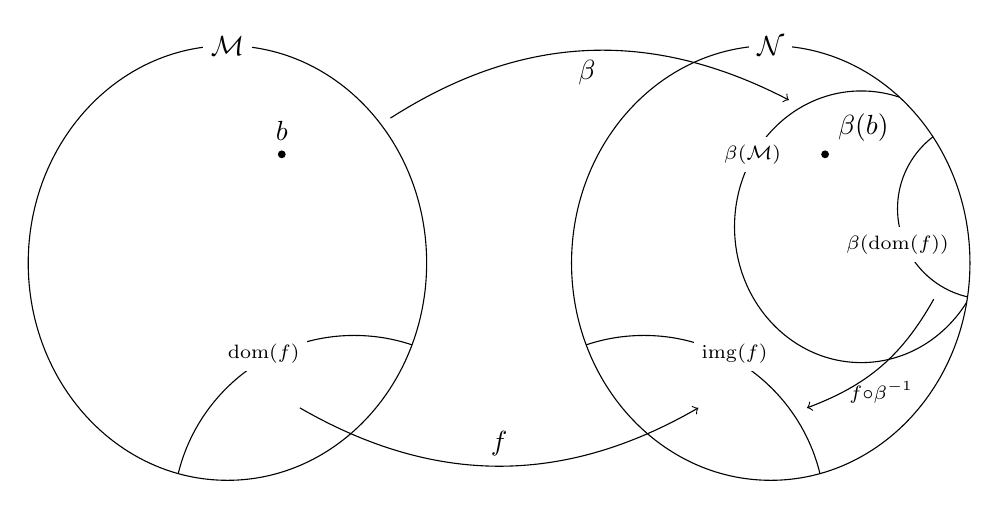
\begin{tikzpicture}[scale=2.3, gaplabel/.style={fill=white, rectangle, inner sep=1mm}]
      \draw (-1.5,0) circle [x radius=1.1cm, y radius=1.2cm];
      \node [gaplabel] at (-1.5,1.2) {$\mathcal{M}$};
      \draw (1.5,0) circle [x radius=1.1cm, y radius=1.2cm];
      \node [gaplabel] at (1.5,1.2) {$\mathcal{N}$};
      \begin{scope}
        \clip (-1.5,0) circle [x radius=1.1cm, y radius=1.2cm];
        \draw (-0.8,-1.4) circle [radius=1cm];
        \node [fill=black, inner sep=1pt, circle, label=above:$b$] (b) at (-1.2,0.6) {};
        \node [gaplabel] at (-1.3,-0.5) {$\scriptstyle\dom(f)$};
      \end{scope}
      \begin{scope}
        \clip (1.5,0) circle [x radius=1.1cm, y radius=1.2cm];
        \draw (0.8,-1.4) circle [radius=1cm];
        \draw (2, 0.2) circle [x radius=0.7cm, y radius=0.75cm];
        \draw (2.7, 0.3) circle [radius=0.5cm];
        \node [fill=black, inner sep=1pt, circle, label=above right:$\beta(b)$] (c) at (1.8,0.6) {};
        \begin{scope}[every node/.style={gaplabel}]
          \node at (1.3,-0.5) {$\scriptstyle\img(f)$};
          \node at (1.4, 0.6) {$\scriptstyle\beta(\mathcal{M})$};
          \node at (2.2, 0.1) {$\scriptstyle\beta(\dom(f))$};
        \end{scope}
      \end{scope}

      \draw[->] (-1.1,-0.8) to[bend right] node[midway, above] {$f$} (1.1,-0.8);
      \draw[->] (-0.6,0.8) to[bend left] node[midway, below] {$\beta$} (1.6,0.9);
      \draw[->] (2.4,-0.2) to[bend left=20] node[midway, below=2] {$\scriptstyle f \circ \beta^{-1}$} (1.7, -0.8);
    \end{tikzpicture}
  \end{center}
  Then the map $f \circ \beta^{-1}: \beta(\dom(f)) \to \img(f)$ is elementary.
  By \hyperlink{def:homogeneous}{homogeneity}, there is $\alpha \in \hyperlink{def:aut}{\Aut}(\mathcal{N})$ such that $f \circ \beta^{-1} \subseteq \alpha$.
  Then $f \cup \{\langle b, \alpha(\beta(b))\}$ is elementary (it is a restriction of $\alpha \circ \beta$).
\end{proof}
\begin{ndef}[Orbit, defined set]\label{def:6.11}
  \hypertarget{def:orbit}Let $\bar{a}$ be a tuple in $\mathcal{N}$ and $A \subseteq N$.
  The \named{orbit} of $\bar{a}$ over $A$ is the set
  \begin{equation*}
    O_\mathcal{N} (\bar{a}/A) = \set{\alpha(\bar{a}) | \alpha \in \hyperlink{def:aut}{\Aut(\mathcal{N}/A)}}.
  \end{equation*}
  \hypertarget{def:setdef}If $\varphi(\bar{x})$ is an \hyperlink{def:la}{$L(A)$-formula}, then
  \begin{equation*}
    \varphi(\mathcal{N}) \coloneqq \set{\bar{a} \in N^{\lvert\bar{x}\rvert} | \mathcal{N} \models \varphi(\bar{a})}
  \end{equation*}
  is the \textbf{set defined by $\varphi(\bar{x})$}.
  A set is \named{definable} over $A$ if it is defined by some $L(A)$-formula.
  There are analogous notions of a type defining a set, and a set being type-definable.
\end{ndef}
\begin{nremark}\label{rem:6.12}
  If\marginnote{\emph{Lecture 12}} $\bar{a}$, $\bar{b}$ are tuples in $\mathcal{N}$ of the same length, and $A\subseteq N$, then the following are equivalent.
  \begin{enumerate}[label=(\roman*)]
    \item $\hyperlink{def:tp}{\tp_{\mathcal{N}}(\bar{a}/A)}= \tp_{\mathcal{N}}(\bar{b}/A)$
    \item $ \set{a_i\mapsto b_i|i < |\bar{a}|}\cup\text{id}_A $ is an \hyperlink{def:el}{elementary map} from $\mathcal{N}$ to $\mathcal{N}$
  \end{enumerate}
\end{nremark}
\begin{nprop}\label{prop:6.13}
  Let $ \mathcal{N} $ be \hyperlink{def:homogeneous}{$\lambda$-homogeneous}, $A\subseteq N$, with $|A|<\lambda$ and let $\bar{a}$ a tuple in $\mathcal{N}$ such that $|\bar{a}|<\lambda$.
  Then
  \begin{equation*}\hyperlink{def:orbit}{O_{\mathcal{N}}(\bar{a}/A)}=\hyperlink{def:setdef}{p(\mathcal{N})}\end{equation*}
  where $p(\bar{x})=\hyperlink{def:tp}{\tp_{\mathcal{N}}(\bar{a}/A)}$.
\end{nprop}
\begin{proof}
  If $\alpha(\bar{a})=\bar{b}$, where $\alpha\in\hyperlink{def:aut}{\Aut(\mathcal{N}/A)}$, then $\hyperlink{def:tp}{\tp_{\mathcal{N}}(\bar{a}/A)}=\tp_{\mathcal{N}}(\bar{b}/A) $.

  If $\tp_{\mathcal{N}}(\bar{a}/A)=\tp_{\mathcal{N}}(\bar{b}/A)$, then $\set{\langle a_i, b_i \rangle | i < |\bar{a}|} \cup \operatorname{id}_A$ is \hyperlink{def:elmap}{elementary}, and by \hyperlink{def:homogeneous}{homogeneity} it extends to $\alpha\in\Aut(\mathcal{N})$, and in particular $\alpha \in \Aut(\mathcal{N}/A)$.
\end{proof}

\clearpage
\section{The Monster Model}
\hypertarget{def:monster}Given a \hyperlink{def:complete}{complete theory} $T$ with an infinite \hyperlink{def:model}{model},
we work in a \hyperlink{def:sat}{saturated} \hyperlink{def:str}{structure} $\mathcal{U}$ (sometimes denoted $\mathbb{M}$) that is a model of $T$, which is sufficiently large such that any other model of $T$ we might be interested in is an \hyperlink{def:elsubs}{elementary substructure} of $\mathcal{U}$.
($\mathcal{U}$ is an expository device - see Tent/Ziegler for more details, also Marker).

\begin{ndef}[Terminology and conventions]\label{def:7.1}
  When working in $\mathcal{U}$, we say
  \begin{itemize}
    \item `$\varphi(\bar{x})$ \textbf{holds}' to mean that $\mathcal{U}\hyperlink{def:models}{\models}\forall \bar{x} \;\varphi(\bar{x})$
    \item `$\varphi(\bar{x})$ is \textbf{consistent}' to mean $\mathcal{U}\models\exists\bar{x}\;\varphi(\bar{x})$
    \item `the type $p(\bar{x})$ is \textbf{consistent}/\textbf{satisfiable}' to mean $\mathcal{U}\models\exists\bar{x}\;p(\bar{x})$
    \item A cardinality $\lambda$ is \hypertarget{def:small}{\named{small}} if $\lambda< |U|$ (usually denote $|U|$ by $\kappa$)
    \item a \textbf{model} is some $\mathcal{M}\preccurlyeq\mathcal{U}$ such that $|M|$ is small
  \end{itemize}
  Conventions:
  \begin{itemize}
    \item all tuples assumed to have small length, unless specified otherwise
    \item \hyperlink{def:form}{formulas} have parameters in $U$
    \item \hyperlink{def:type}{types} have parameters in small sets
    \item \hyperlink{def:setdef}{definable sets} have the form $\varphi(U)$ for some $L(U)$-formula $\varphi(\bar{x})$
    \item \hyperlink{def:setdef}{type definable sets} have the form $p(U)$ for some type $ p(\bar{x},A)$ where $|A| < \kappa$.
    \item Orbits and types of tuples are within $\mathcal{U}$, so $\tp(\bar{a}/A)$ means $\tp_{\mathcal{U}}(\bar{a}/A)$,
      \begin{equation*} O(\bar{a}/A)=O_{\mathcal{U}}(\bar{a}/A) \end{equation*}
    \item If $p(\bar{x})$, $q(\bar{x})$ are \hyperlink{def:type}{types}, we write $p(\bar{x})\to q(\bar{x})$ to mean $p(\mathcal{N})\subseteq q(\mathcal{N})$ (think of $p(\bar{x})$ as an infinite conjunction of formulas)
  \end{itemize}
\end{ndef}
\begin{nfact}\label{fact:7.2}
  Let $p(\bar{x})$ be a \hyperlink{def:type}{satisfiable} \hyperlink{def:typeparam}{$L(A)$-type}, and $q(\bar{x})$ a satisfiable $L(B)$-type, such that
  \begin{equation*}p(\bar{x})\to \lnot q(\bar{x})\end{equation*}
  (explicitly, $p(\bar{x})$ and $q(\bar{x})$ have no common realisations).

  Then there are $\varphi_i(\bar{x}) \in p(\bar{x})$ and $\psi_i(\bar{x}) \in q(\bar{x})$ such that
  \begin{equation*} \bigwedge_{i=1}^n\varphi_i(\bar{x})\to \lnot \left(\bigwedge_{i=1}^m\psi_i(\bar{x})\right).\end{equation*}
\end{nfact}
\begin{proof}
  $p(\bar{x})\cup q(\bar{x})$ is not \hyperlink{def:type}{realized} in $\mathcal{U}$.
  By \hyperlink{def:sat}{saturation} of $\mathcal{U}$, $p(\bar{x}) \cup q(\bar{x})$ is not \hyperlink{def:type}{finitely satisfiable},
  hence there exist finite subsets
  $\{\varphi_1(\bar{x}), \dotsc, \varphi_n(\bar{x})\} \subseteq p(\bar{x}),$
  $\{\psi_1(\bar{x}), \dotsc, \psi_n(\bar{x})\}\subseteq q(\bar{x})$
  such that their union is not satisfiable.
  Then
  \begin{equation*} \bigwedge \varphi_i(\bar{x}) \to \lnot\left(\bigwedge \psi_i(\bar{x}) \right). \qedhere \end{equation*}
\end{proof}
\begin{nremark}\label{rem:7.3}
  Let $ \varphi(\mathcal{U},\bar{b}) $ be such that $\varphi(\bar{x},\bar{z})$ is an \hyperlink{def:form}{$L$-formula}, $\bar{b}\in \mathcal{U}^{|\bar{z}|} $.
  If $ \alpha\in\hyperlink{def:aut}{\Aut(\mathcal{U})} $, then
  \begin{align*}
    \alpha[\varphi(\mathcal{U},\bar{b})] &= \set{\alpha(\bar{a})|\varphi(\bar{a},\bar{b}), \bar{a} \in \mathcal{U}^{|\bar{x}|}}\\
                                         &= \set{\alpha(\bar{a})|\varphi(\alpha(\bar{a}),\alpha(\bar{b})), \bar{a} \in \mathcal{U}^{|\bar{x}|}}\\
                                         &= \varphi(\mathcal{U},\alpha(\bar{b}))
  \end{align*}
  So $\Aut(\mathcal{U})$ acts on the definable sets in a natural way. (Similarly for the type-definable sets)
\end{nremark}
\begin{ndef}[Invariant]\label{def:7.4}
  \hypertarget{def:inv}A set $D\subseteq \mathcal{U}$ is \named{invariant} under $\hyperlink{def:aut}{\Aut}(\mathcal{U}/A)$ (\textbf{invariant over $A$})
  if $\hyperlink{def:setdef}{\alpha(D)}=D$ for every $\alpha\in\Aut(\mathcal{U}/A)$.

  Equivalently, for all $\bar{a}\in D$, $\hyperlink{def:orbit}{O(\bar{a}/A)}\subseteq D$.

  If $\bar{a}\in D$, $q(\bar{x})=\tp(\bar{a}/A)$ and $\bar{b}\models q(\bar{x})$, then $\bar{b}\in D$.
  ($\tp(\bar{b}/A) =\tp(\bar{a}/A)$, so there is $\alpha\in\Aut(\mathcal{U}/A)$ s.t.\ $\alpha(\bar{a})=\bar{b}$ by \hyperlink{def:homogeneous}{homogeneity} of $\mathcal{U}$).
  Hence we could also define invariance over $A$ as
  \begin{equation*}
  \forall \bar{a}\in D,\qquad \bar{b}\hyperlink{def:eleqa}{\equiv_A}\bar{a}\implies \bar{b}\in D.
  \end{equation*}
\end{ndef}
\begin{nprop}\label{prop:7.5}
  Let $\varphi(\bar{x})$ be an \hyperlink{def:la}{$L(U)$}-\hyperlink{def:form}{formula}, then the following are equivalent:
  \begin{enumerate}[label=(\roman*)]
    \item $\varphi(\bar{x})$ is equivalent to some $L(A)$-formula $\psi(\bar{x})$
    \item $ \varphi(\mathcal{U}) $ is \hyperlink{def:inv}{invariant} over $A$
  \end{enumerate}
\end{nprop}
\begin{proof}
  (i) $\Rightarrow$ (ii) is clear.

  (ii) $\Rightarrow$ (i): Let $\varphi(\bar{x},\bar{z})$ be an \hyperlink{def:form}{$L$-formula} such that $\varphi(\mathcal{U},\bar{b})$ is \hyperlink{def:inv}{invariant} over $A$, for suitable $ \bar{b} \in U^{|\bar{z}|}$.

  Let $q(\bar{z})$ be the \hyperlink{def:type}{type} $\tp(\bar{b}/A)$.
  If $ \bar{c}\hyperlink{def:models}{\models} q(\bar{z}) $, then there is $ \alpha\in\hyperlink{def:aut}{\Aut(\mathcal{U}/A)}$
  such that $\alpha(\bar{b})=\bar{c}$.
  Then
    \begin{align*}
      \varphi(\mathcal{U},\bar{c})&=\alpha(\varphi(\mathcal{U},\bar{b}))\qquad\text{by \cref{rem:7.3}} \\
                                       &= \varphi(\mathcal{U},\bar{b})\qquad\text{by invariance}
    \end{align*}
  Hence
  \begin{equation*}
    q(\bar{z})\to \forall\bar{x}\;(\varphi(\bar{x},\bar{z})\leftrightarrow\varphi(\bar{x},\bar{b})).
  \end{equation*}
  By an argument similar to \cref{fact:7.2},
  there is $\theta(\bar{z})\in q(\bar{z})$ such that $\theta(\bar{z})\to\forall\bar{x}\;(\varphi(\bar{x},\bar{z})\leftrightarrow\varphi(\bar{x},\bar{b}))$.
  Then $\theta(\bar{z})$ is an $L(A)$-formula and $\exists z\;[\theta(\bar{z})\land\varphi(\bar{x},\bar{z})]$ defines $ \varphi(\mathcal{U},\bar{b}) $.
\end{proof}
\begin{ndef}\label{def:7.6}
  \marginnote{\emph{Lecture 13}}\hypertarget{def:upe}An injective map $p: A \subseteq \mathcal{M} \to \mathcal{N}$ is a \named{partial embedding} if for all tuples in $A = \dom(p)$, $p$ satisfies conditions (i), (ii), (iii) in \cref{def:1.5}.
\end{ndef}
Idea: a \hyperlink{def:upe}{partial embedding} preserves quantifier-free \hyperlink{def:form}{formulas}.
\begin{nprop}\label{prop:7.7}
  Let $\varphi(\bar{x})$ be an \hyperlink{def:form}{$L$-formula}. The following are equivalent:
  \begin{enumerate}[label=(\roman*)]
    \item there is $\psi(\bar{x})$, a quantifier-free $L$-formula such that
      \begin{equation*}
        \mathcal{U} \hyperlink{def:models}{\models} \forall x\; [\varphi(\bar{x}) \leftrightarrow \psi(\bar{x})].
      \end{equation*}
    \item for all \hyperlink{def:upe}{partial embeddings} $p: \mathcal{U} \to \mathcal{U}$, for all $\bar{a}$ from $\dom(\bar{p})$,
      \begin{equation*}
        \varphi(\bar{a}) \leftrightarrow \varphi(p(\bar{a}))
      \end{equation*}
  \end{enumerate}
\end{nprop}
\begin{proof}
  (i) $\Rightarrow$ (ii): clear.

  (ii) $\Rightarrow$ (i). For $\bar{a} \in U$, set
  \begin{equation*}
    \hypertarget{def:qftp}\qftp(\bar{a}) \coloneqq \set{\psi(\bar{x}) | \psi(\bar{a}) \text{ and } \psi(\bar{x}) \text{ is quantifier free}}. % fix this
  \end{equation*}
  Let
  \begin{equation*}
  D = \set{q(\bar{x}) | q(\bar{x}) = \qftp(\bar{a}) \text{ for some }\bar{a} \text{ such that } \varphi(\bar{a})}.
  \end{equation*}
  Claim: $\varphi(U) = \bigcup_{q(\bar{x}) \in D} q(U)$.

  By (an argument similar to) \cref{fact:7.2}, there is $\theta_q(\bar{x})$ in $q(\bar{x})$ a finite conjunction of formulas such that $\theta_q(\bar{x}) \to \varphi(x)$.
  So we have
  \begin{equation*}
    \varphi(\bar{x}) \leftrightarrow \bigvee_{q(\bar{x}) \in D} \{\theta_q(\bar{x})\}.
  \end{equation*}
  By \cref{fact:7.2}, there are $\psi_{q_1}(\bar{x}), \dotsc, \psi_{q_m}(\bar{x})$ such that
  \begin{equation*}
    \varphi(\bar{x}) \leftrightarrow \bigvee_{i=1}^n \psi_{q_i}(\bar{x}).
  \end{equation*}
  So $\bigvee \psi_{q_i}(\bar{x})$ is the required quantifier-free formula.
\end{proof}
\begin{ndef}\label{def:7.8}
  \hypertarget{def:qe}An $L$-theory $T$ has \named{quantifier elimination} if for every $L$-formula $\varphi(\bar{x})$ there is $\psi(\bar{x})$ quantifier free such that
  \begin{equation*}
    T \vdash \forall \bar{x}\; (\varphi(\bar{x}) \leftrightarrow \psi(\bar{x})).
  \end{equation*}
\end{ndef}
\begin{nthm}
  Let $T$ be a complete theory with an infinite model. Then the following are equivalent:
  \begin{enumerate}[label=(\roman*)]
    \item $T$ has \hyperlink{def:qe}{quantifier elimination}
    \item every $p: \mathcal{U} \to \mathcal{U}$ \hyperlink{def:upe}{partial embedding} is \hyperlink{def:el}{elementary}
    \item If $p: \mathcal{U} \to \mathcal{U}$ is partial embedding and $|\dom p| < |\mathcal{U}|$ and $b \in \mathcal{U}$, then there is a partial embedding $\hat{p} \supseteq p$ such that $b \in \dom \hat{p}$.
  \end{enumerate}
\end{nthm}
\begin{proof}
  (i) $\Leftrightarrow$ (ii). Follows from \cref{prop:7.7}.

  (ii) $\Rightarrow$ (iii). If $p: \mathcal{U} \to \mathcal{U}$ is a \hyperlink{def:upe}{partial embedding}, then it is \hyperlink{def:elmap}{elementary}.
  Let $b \in \mathcal{U}$.
  By \hyperlink{def:homogeneous}{homogeneity} of $\mathcal{U}$, there is $\alpha \in \Aut(\mathcal{U})$ such that $p \subseteq \alpha$, and so $p \cup \{\langle b, \alpha(b) \rangle \}$ is the required extension of $p$.

  %(iii) $\Rightarrow$ (ii). Prove that if $p: \mathcal{U} \to \mathcal{U}$ is partial embedding, then any finite restriction $p_0$ of $p$ is an elementary map.
  %Idea: Let $\mathcal{M} \supseteq \dom(p_0)$, $\mathcal{N} \supseteq \img(p_0)$ such that $|\mathcal{M}| = |\mathcal{N}|$, and extend $p_0$ to $\beta: \mathcal{M} \to \mathcal{N}$ by back-and-forth (use saturation of $\mathcal{U}$).
  (iii) $\Rightarrow$ (ii). Let $p: \mathcal{U} \to \mathcal{U}$ be a partial embedding.
  Consider $p_0 \subseteq p$, $p_0$ finite or small. Use property (iii) and saturation to extend $p_0$ to $\alpha \in \Aut(U)$ by back and forth.
\end{proof}
\begin{remark}
  There is a fourth condition equivalent to (i), (ii), (iii):
  \begin{enumerate}[label=(\roman*)]\setcounter{enumi}{3}
    \item for every finite partial embedding $p: \mathcal{U} \to \mathcal{U}$ and $b \in \mathcal{U}$ there is $\hat{p} \supseteq p$, a partial embedding such that $b \in \dom(\hat{p})$.
  \end{enumerate}

  Proof: Later, exercise.
\end{remark}

This gives \hyperlink{def:qe}{quantifier elimination} for $T_{\text{rg}}$ and $T_{\text{dlo}}$.
\begin{remark}
  If $T$ has \hyperlink{def:qe}{quantifier elimination} and $\mathcal{M} \models T$, any \hyperlink{def:subs}{substructure} of $\mathcal{M}$ is an \hyperlink{def:elsubs}{elementary substructure} ($T$ is `model-complete').
\end{remark}
\begin{ndef}
  \hypertarget{def:def}An element $a \in \mathcal{U}$ is \textbf{definable} over $A \subseteq U$ if there is an $L(A)$-formula $\varphi(x)$ such that $\varphi(U) = \{a\}$. (In particular, any element of $A$ is definable over $A$; $x=a$ for $a \in A$).

  \hypertarget{def:alg}An element $a \in \mathcal{U}$ is \textbf{algebraic} over $A \subseteq U$ if there is an $L(A)$-formula $\varphi(x)$ such that $|\varphi(U)| < \omega$ and $a \in \varphi(\mathcal{U})$.

  The \textbf{definable closure} of $A$ is
  \begin{equation*}
    \dcl(A) = \set{a \in \mathcal{U} | a \text{ definable over }A}
  \end{equation*}
  and the \textbf{algebraic closure} of $A$ is
  \begin{equation*}
    \acl(A) = \set{a \in \mathcal{U} | a \text{ algebraic over }A}.
  \end{equation*}
\end{ndef}
\begin{nprop}\label{prop:7.11}
  For $a \in \mathcal{U}$ and $A \subseteq \mathcal{U}$, the following are equivalent
  \begin{enumerate}[label=(\roman*)]
    \item $a \in \hyperlink{def:def}{\dcl(A)}$
    \item $\hyperlink{def:orbit}{O(a/A)} = \{a\}$. % Orb(a/A)
  \end{enumerate}
\end{nprop}
\begin{proof}
  $a \in \hyperlink{def:def}{\dcl(A)}$ iff there is $\varphi(x) \in \hyperlink{def:la}{L(A)}$ such that $\varphi(U) = \{a\}$.
  By \cref{prop:7.5} this is equivalent to \hyperlink{def:inv}{invariance} under $\hyperlink{def:aut}{\Aut}(U/A)$.
\end{proof}
\begin{nthm}\label{thm:7.12}
  Let $A \subseteq \U$, $a \in \U$, the following are equivalent:
  \begin{enumerate}[label=(\roman*)]
    \item $a \in \hyperlink{def:alg}{\acl(A)}$
    \item $|\hyperlink{def:orbit}{O(a/A)}| < \omega$
    \item $a \in \mathcal{M}$ for any \hyperlink{def:model}{model} $\mathcal{M}$ which contains $A$.
  \end{enumerate}
\end{nthm}
\begin{proof}
  \marginnote{\emph{Lecture 14}}
  (i) $\Rightarrow$ (ii). If $a \in \hyperlink{def:alg}{\acl}(A)$, then there is an \hyperlink{def:la}{$L(A)$}-\hyperlink{def:form}{formula} $\varphi(x)$ such that $\varphi(a)$ holds and $|\varphi(U)| < \omega$.
  But $\varphi(U)$ is \hyperlink{def:inv}{invariant} over $A$, and so $O(a/A) \subseteq \varphi(U)$, and so $|\mathcal{O}(a/A)| < \omega$.

  (ii) $\Rightarrow$ (i). If $|\hyperlink{def:orbit}{O(a/A)}| < \omega$, then $O(a/A)$ is \hyperlink{def:def}{definable} by $\bigvee_{i=1}^n (x = a_i)$ where $O(a/A) = \{a_1, \dotsc, a_n\}$.
  Also $O(a/A)$ is \hyperlink{def:inv}{invariant} over $A$, so by \cref{prop:7.5}, there is an $L(A)$-formula $\varphi(x)$ that defines $O(a/A)$.

  (i) $\Rightarrow$ (iii). $a \in \acl(A)$, so there is $\varphi(x)$, an $L(A)$-formula such that there is $n \in \omega\setminus\{0\}$ with
  \begin{equation*}
    \varphi(a) \wedge \exists^{\leq n} x \; \varphi(x).
  \end{equation*}
  Then by \hyperlink{def:elmap}{elementarity}, $\varphi(a) \wedge \exists^{\leq n} x \; \varphi(x)$ holds in every $\mathcal{M} \supseteq A$, and the $n$ realizations of $\varphi(x)$ in $\mathcal{U}$ must coincide with the realizations in $\mathcal{M}$.
  Therefore $a \in \mathcal{M}$.

  (iii) $\Rightarrow$ (i). Suppose $a \notin \acl(A)$, let $p(x) = \tp(a/A)$. Then for $\varphi(x) \in p(x)$, $|\varphi(\mathcal{U})| \geq \omega$.
  Then from sheet 2, $|p(\mathcal{U})| \geq \omega$.
  By an argument similar to the one in exercise 7 on sheet 2, $|p(\mathcal{U})| = |\mathcal{U}|$.

  Let $\mathcal{M} \supseteq A$, then $p(\mathcal{U}) \setminus \mathcal{M} \neq \emptyset$.
  So there is $b \in p(\mathcal{U}) \setminus \mathcal{M}$.
  Since $\hyperlink{def:tp}{\tp}(a/A) = \tp(b/A)$, there is $\alpha \in \hyperlink{def:aut}{\Aut}(\mathcal{U}/A)$ such that $\alpha(b) = a$.

  But then $\alpha[\mathcal{M}]$ is a \hyperlink{def:model}{model} that contains $A$, but $a \notin \alpha[\mathcal{M}]$ while $a = \alpha(b)$.
\end{proof}

\begin{nprop}\label{prop:7.13}
  Let $a \in \mathcal{U}$, $A \subseteq \mathcal{U}$. Then:
  \begin{enumerate}[label=(\roman*)]
    \item if $a \in \hyperlink{def:alg}{\acl}(A)$, then there is finite $A_0 \subseteq A$ such that $a \in \acl(A_0)$.
    \item if $A \subseteq B$, then $\acl(A) \subseteq \acl(B)$.
    \item $\acl(A) = \acl(\acl(A))$
    \item $A \subseteq \acl(A)$.
    \item $\acl(A) = \bigcap_{A \subseteq \mathcal{M}} \mathcal{M}$
      where $\mathcal{M}$ is a \hyperlink{def:small}{small} \hyperlink{def:elsubs}{elementary substructure} of $\mathcal{U}$.
  \end{enumerate}
\end{nprop}
\begin{proof}\leavevmode
  \begin{enumerate}[label=(\roman*)]
    \item[(iv)] $a \in A$ is \hyperlink{def:def}{definable} over $A$, hence \hyperlink{def:alg}{algebraic}.
    \item[(iii)] $\hyperlink{def:alg}{\acl}(A) \subseteq \acl(\acl(A))$ by monotonicity.
      For $\supseteq$, let $a \in \acl(\acl(A))$. By \cref{thm:7.12}, $a \in \mathcal{M}$ for every $\mathcal{M} \supseteq \acl(A)$.
      But $\acl(A) \subseteq \mathcal{M} \iff A \subseteq \mathcal{M}$, so $a \in \mathcal{M}$ for every $\mathcal{M} \supseteq A$, i.e.\ $a \in \acl(A)$.
      \item[(v)] follows from \cref{thm:7.12}. \qedhere
  \end{enumerate}
\end{proof}
\begin{nprop}\label{prop:7.14}
  If $\beta\in \hyperlink{def:aut}{\Aut(\mathcal{U})}$, $A \subseteq \mathcal{U}$, then $\beta[\hyperlink{def:alg}{\acl}(A)] = \acl(\beta[A])$.
\end{nprop}
\begin{proof}
  $\subseteq$: Let $a \in \hyperlink{def:alg}{\acl}(A)$, let $\varphi(x, \bar{z})$ be an $L$-\hyperlink{def:form}{formula} such that $\varphi(a, \bar{b})$ holds for $\bar{b}$ in $A$ and $|\varphi(U, \bar{b}) < \omega$.
  Then $\varphi(\beta(a), \beta(\bar{b}))$ holds, $|\varphi(U, \beta(\bar{b}))|<\omega$, and so $\beta(a)$ is \hyperlink{def:alg}{algebraic} over $\beta[\bar{b}]$.

  The same proof with $\beta^{-1}$ in place of $\beta$ and $\beta[A]$ in place of $A$ shows $\supseteq$.
\end{proof}

\clearpage
\section{Strongly Minimal Theories}
\begin{ndef}[Cofinite]\label{def:8.1}
  \hypertarget{def:cofinite}For $\mathcal{M}$ a \hyperlink{def:str}{structure}, $A \subseteq M$ is \named{cofinite} if $M \setminus A$ is finite.
\end{ndef}
\begin{nremark}
  Finite and \hyperlink{def:cofinite}{cofinite} sets are \hyperlink{def:def}{definable} in every \hyperlink{def:str}{structure}.
\end{nremark}
In this chapter, we'll look at \hyperlink{def:str}{structures} where these are the only \hyperlink{def:def}{definable} sets.
\begin{ndef}[Minimality, strong minimality]\hypertarget{def:minimal}
  A \hyperlink{def:str}{structure} $\mathcal{M}$ is \named{minimal} if all its \hyperlink{def:def}{definable} subsets are finite or \hyperlink{def:cofinite}{cofinite}.
  $\mathcal{M}$ is \named{strongly minimal} if it is minimal and all its elementary extensions are minimal.

  If $T$ is a \hyperlink{def:consistent}{consistent} theory without finite \hyperlink{def:models}{models}, $T$ is \textbf{strongly minimal} if for every formula $\varphi(x, \bar{z})$ there is $n \in \omega \setminus \{0\}$ such that
  \begin{equation*}
    T \vdash \forall \bar{z} \; [\exists^{\leq n} x \; \varphi(x, \bar{z}) \lor \exists^{\leq n} x \; \neg \varphi(x, \bar{z})].
  \end{equation*}
\end{ndef}
\begin{eg}
  Take $L = \{E\}$, a binary relation, let $\mathcal{M}$ be the $L$-\hyperlink{def:str}{structure} where $E$ is an equivalence relation with exactly one class of size $n$ for all $n \in \omega$ and no infinite classes.
  Then can show $\mathcal{M}$ is \hyperlink{def:minimal}{minimal} (can only say things like `$x$ is in the same class as a').

  But, there is $\mathcal{N} \hyperlink{def:elsubs}{\succcurlyeq} \mathcal{M}$ where $\mathcal{N}$ has an infinite class.
  Then if the equivalence class of $a \in \mathcal{N}$ is infinite, the set defined by $E(x,a)$ is infinite/coinfinite, so $\M$ is not \hyperlink{def:minimal}{strongly minimal}.
\end{eg}
(Remark: \hyperlink{def:minimal}{strongly minimal} \hyperlink{def:ltheory}{theories} have \hyperlink{def:monster}{monster models}).
From now on: $T$ is strongly minimal, \hyperlink{def:complete}{complete}, and has an infinite \hyperlink{def:model}{model}.
\begin{ndef}[Independence]\label{def:8.4}
  \hypertarget{def:indep}Let $a \in \mathcal{U}$, $B \subseteq \mathcal{U}$. Then $a$ is \named{independent} from $B$ if $a \notin \hyperlink{def:alg}{\acl}(B)$.
  The set $B$ is \textbf{independent} if for all $a \in B$, $a \notin \acl(B\setminus\{a\})$.
\end{ndef}
% new lecture
\begin{eg}\leavevmode
  \begin{itemize}
    \item \marginnote{\emph{Lecture 15}}\hypertarget{def:vsk}Vector spaces. Fix an infinite field $K$, and use $L = \{+, -, \vec{0}, \{\lambda\}_{\lambda \in K}\}$, where $\lambda$ are unary functions (for scalar multiplication).
      The theory of vector spaces over $K$, $T_{VSK}$ includes:
      \begin{itemize}
        \item axioms in $\{+,-,\vec{0}\}$ for abelian group
        \item axiom schemata for scalar multiplication:
          \begin{itemize}
            \item $\forall x y \; [\lambda (x+y) = \lambda x + \lambda y]$ for each $\lambda \in K$, $\lambda x$ means $\lambda(x)$.
            \item $\vdots$
            \item $\forall x \; [1 x = x]$ (since $1 \in K$).
            \item $\exists x \; (x \neq \vec{0})$.
          \end{itemize}
      \end{itemize}
      Then it can be shown $T_{VSK}$ is \hyperlink{def:complete}{complete} and has \hyperlink{def:qe}{quantifier elimination}.

      \hyperlink{def:atomform}{Atomic formulas} express equality of linear combinations, any atomic formula in one variable and with parameters is equivalent to `$\lambda x = a$', so atomic formulas in one variable define singletons.
      Quantifier-free formulas in one variable and with parameters define sets that are either finite or \hyperlink{def:cofinite}{cofinite}.

      By \hyperlink{def:qe}{quantifier elimination}, $T_{VSK}$ is \hyperlink{def:minimal}{strongly minimal}.
      Also, $\acl(A) = \langle A \rangle$, the linear span, and $a$ is \hyperlink{def:indep}{independent} from $A$ if $a$ is linearly independent from $A$, and $A$ is independent if it is linearly independent.

    \item \hypertarget{def:acf}Fields. Take $L_{\text{ring}} = \{+, \cdot , - , 0, 1\}$. Then $ACF$ is the theory that includes
      \begin{itemize}
        \item axioms for abelian group in $\{+,-,0\}$
        \item axioms for multiplicative monoids in $\{\cdot, 1\}$
        \item $\forall x y z \; [x \cdot (y + z) = x \cdot y + x \cdot z]$
        \item $\forall x \; [x = 0 \lor \exists y \; (x\cdot y ) = 1]$
        \item $0 \neq 1$
        \item axioms for algebraic closure: for all $n$,
          \begin{equation*}
            \forall x_0 \dotsm x_n \; \exists y \; [x_n y^n + \dotsb + x_1 y + x_0 = 0].
          \end{equation*}
      \end{itemize}
      If
      \begin{equation*}\chi_p \equiv \underbrace{1 + 1 + \dotsb + 1}_{p \text{ times}} = 0,\end{equation*}
      for $p$ prime, then $ACF \cup \{\chi_p\} \eqqcolon ACF_p$, which can be shown to be \hyperlink{def:complete}{complete} and have \hyperlink{def:qe}{quantifier elimination}.
      By adding $\{\lnot \chi_n \mid n \in \omega\}$ to $ACF$, get $ACF_0$ (also complete with quantifier elimination).

      Now, atomic formulas with parameters are polynomial equations.
      An atomic formula with one variable (and parameters in $A$) is equivalent to $p(x) = 0$, where $p(x)$ is a polynomial in the subfield generated by $A$.
      So such atomic formulas define finite sets, and quantifier free formulas define finite or cofinite sets, and so by quantifier elimination, $ACF_p$ ($ACF_0$) is strongly minimal.
      If $a \in \mathcal{M} \hyperlink{def:models}{\models} ACF_p$, $A \subseteq \mathcal{M}$, then $a \in \hyperlink{def:alg}{\acl}(A)$ if $a$ is algebraic over the field generated by $A$.
  \end{itemize}
\end{eg}
\begin{notation}
  \hypertarget{def:algnot}We write $\acl(a,B)$ for $\hyperlink{def:alg}{\acl}(\{a\} \cup B)$ and $\acl(B\setminus a)$ for $\acl(B \setminus \{a\})$.
\end{notation}
\begin{nthm}\label{thm:8.5}
  Let $B \subseteq \mathcal{U}$, and $a,b \notin \acl(B)$. ($a,b \in \mathcal{U} \setminus \acl(B)$).
  Then
  \begin{equation*}
    b \in \hyperlink{def:algnot}{\acl}(a,B) \iff a \in \acl(b,B).
  \end{equation*}
\end{nthm}
\begin{proof}
  Let $a,b \in \hyperlink{def:alg}{\acl}(B)$. Assume $b \notin \hyperlink{def:algnot}{\acl(a,B)}$ and $a \in \acl(b,B)$.
  Let $\varphi(x,y)$ be an $L(B)$-\hyperlink{def:form}{formula} such that for some $n$,
  \begin{equation*}
    \varphi(a,b) \land \exists^{\leq n} x \; \varphi(x,b).
  \end{equation*}
  Since $b \notin \acl(a,B)$
  \begin{equation*}
    \psi(a,y) \coloneqq \varphi(a,y) \land \exists^{\leq n} x \; \varphi(x,y)
  \end{equation*}
  is such that $|\psi(a,\mathcal{U})| \geq \omega$.
  By question 7, example sheet 2, $|\psi(a,U)| = |\mathcal{U}|$.
  By \hyperlink{def:minimal}{strong minimality}, $|\neg \psi(a,U)| < \omega$.
  By cardinality considerations, if $\mathcal{M} \supseteq B$, then $\mathcal{M}$ contains $c$ such that $\psi(a,c)$.
  But then $a \in \acl(c,B)$, so $a \in \mathcal{M}$.
  Therefore $a$ is in all \hyperlink{def:model}{models} that contain $B$, so $a \in \acl(B)$ by \cref{thm:7.12}, a contradiction.
\end{proof}
\begin{ndef}[Basis]\label{def:8.6}
  \hypertarget{def:basis}Let $B \subseteq C \subseteq \mathcal{U}$. Then $B$ is a \named{basis} of $C$ if
  \begin{enumerate}[label=(\roman*)]
    \item $B$ is \hyperlink{def:indep}{independent},
    \item $C \subseteq \hyperlink{def:alg}{\acl}(B)$ (or equivalently, $\acl(B) = \acl(C)$).
  \end{enumerate}
\end{ndef}
\begin{nlemma}\label{lem:8.7}
  If $B$ is \hyperlink{def:indep}{independent} and $a \notin \hyperlink{def:alg}{\acl}(B)$, then $\{a\} \cup B$ is independent.
\end{nlemma}
\begin{proof}
  Let $a \notin \hyperlink{def:alg}{\acl}(B)$, and suppose (for contradiction) that $\{a\} \cup B$ is not independent.
  Then there is $b \in B$ such that $b \in \hyperlink{def:algnot}{\acl(a, B\setminus b)}$.
  But $b \notin \acl(B \setminus b)$. Since $a \notin \acl(B \setminus b)$, by \cref{thm:8.5} we have
  \begin{equation*}
    a \in \acl(b, B \setminus b) = \acl(B),
  \end{equation*}
  a contradiction.
\end{proof}
\begin{ncor}\label{cor:8.8}
  If $B \subseteq C$, the following are equivalent:
  \begin{enumerate}[label=(\roman*)]
    \item $B$ is a \hyperlink{def:basis}{basis} of $C$
    \item if $B \subseteq B' \subset C$ and $B'$ is \hyperlink{def:indep}{independent}, then $B = B'$.
  \end{enumerate}
\end{ncor}
\begin{proof}
  By \cref{lem:8.7}.
\end{proof}
\begin{nthm}\label{thm:8.9}
  Let $C \subseteq \U$, then
  \begin{enumerate}[label=(\roman*)]
    \item every \hyperlink{def:indep}{independent} subset $B \subseteq C$ can be extended to a \hyperlink{def:basis}{basis}.
    \item if $A,B$ are bases of $C$, then $|A| = |B|$.
  \end{enumerate}
\end{nthm}
\begin{proof}\leavevmode
  \begin{enumerate}[label=(\roman*)]
    \item If $\langle B_i : i < \lambda \rangle$ is a chain of \hyperlink{def:indep}{independent} sets containing $B$, then $\bigcup_{i < \lambda} B_i$ is independent (by \cref{prop:7.13}(i)).
      By Zorn's lemma, there is a maximal independent subset of $C$ that contains $B$. By \cref{cor:8.8}, that maximal subset is a \hyperlink{def:basis}{basis} of $C$.
    \item \marginnote{\emph{Lecture 16}}Let $|B| \geq \omega$, assume (for contradiction) that $|A| < |B|$.
      Then $a \in A$ is also in $\hyperlink{def:alg}{\acl}(B)$.
      Let $D_a \subseteq B$ be finite such that $a \in \acl(D_a)$. Let $D = \bigcup_{a \in A} D_a$.
      Then $A \subseteq \acl(D)$ and $C \subseteq \acl(D)$, but $|D| < |B|$ contradicting the independence of $B$.

      If $A$ and $B$ are finite, show that $|A| \leq |B|$  (and symmetrically) by using: if there is $a \in A \setminus B$, then there is $b \in B \setminus A$ such that $\{b\} \cup A \setminus \{a\}$ is independent.
      This holds because if $a \in A \setminus B$, then since $a \in \acl(B)$, we have that $B \nsubseteq \acl(A \setminus \{a\})$ (otherwise $A$ is not independent).
      So let $b \in B \setminus \acl(A \setminus a)$.
      Then $\{b\} \cup (A \setminus a)$ is independent by \cref{lem:8.7}.

      Use finite induction argument to get $|A| \leq |B|$. \qedhere
  \end{enumerate}
\end{proof}
\begin{ndef}[Dimension]\label{def:8.10}
  \hypertarget{def:dim}Let $C \subseteq \mathcal{U}$ be \hyperlink{def:alg}{algebraically closed}.
  Then the \named{dimension} of $C$ is $\dim(C) = |A|$ where $A$ is any \hyperlink{def:basis}{basis} of $C$.
\end{ndef}

\begin{nprop}\label{prop:8.11}
  Let $f: \mathcal{U} \to \mathcal{U}$ be \hyperlink{def:upe}{(partial) elementary}.
  Let $b \notin \hyperlink{def:alg}{\acl}(\dom(f))$ and $c \notin \acl(\img(f))$.
  Then $f \cup \{\langle b, c \rangle\}$ is elementary.
\end{nprop}
\begin{proof}
  Let $\bar{a}$ enumerate $\dom(f)$, let $\varphi(x, \bar{a})$ be a formula with parameters in $\bar{a}$.
  Claim: $\varphi(b,\bar{a})) \leftrightarrow \varphi(c, f(\bar{a}))$. Cases:
  \begin{enumerate}
  \item $|\varphi(\mathcal{U}, \bar{a})| < \omega$. Then $|\varphi(\mathcal{U}, f(\bar{a}))| < \omega$.
    Then $b \notin \varphi(\mathcal{U}, \bar{a})$ (because $b \notin \acl(\bar{a})$) and $c \notin \varphi(\mathcal{U}, f(\bar{a}))$.
    Then
    \begin{equation*}
      \lnot \varphi(b, \bar{a}) \land \neg \varphi(c, f(\bar{a})).
    \end{equation*}
  \item $|\varphi(U, \bar{a})| \geq \omega$. Then $|\neg \varphi(\mathcal{U}, \bar{a})| < \omega$, and so
    \begin{equation*}
      \varphi(b, \bar{a}) \land \varphi(c, f(\bar{a})). \qedhere
    \end{equation*}
  \end{enumerate}
\end{proof}
\begin{ncor}\label{cor:8.12}
  Every bijection between \hyperlink{def:indep}{independent} subsets of $\mathcal{U}$ is \hyperlink{def:upe}{elementary}.  \end{ncor}
\begin{proof}
  Pick $A,B \subseteq C$ \hyperlink{def:indep}{independent} and let $f: A \to B$ be any bijection.
  Let $\bar{a}$ enumerate $A$, write $f(a_i) = b_i$.
  Then $a_0 \notin \acl(\emptyset)$ and $b_0 \notin \acl(\emptyset)$ (otherwise $A,B$ not independent). By \cref{prop:8.11}, $\{\langle a_0, b_0 \rangle \}$ is an elementary map.

  At stage $i+1$, $a_{i+1} \notin \acl(a_0, \dotsc, a_i)$ so use the same argument.
\end{proof}

\begin{nremark}\label{rem:8.13}
If $\M \subseteq \U$, then by \cref{prop:7.13}, $\M$ is algebraically closed.
\end{nremark}

\begin{nthm}\label{thm:8.14}
  Suppose that $\M, \N \subseteq \U$ are such that $\hyperlink{def:dim}{\dim}(M) = \dim(N)$, then $\M \hyperlink{def:iso}{\simeq} \N$.
\end{nthm}
\begin{proof}
  Let $A,B$ be \hyperlink{def:basis}{bases} of $\M,\N$ respectively.
  Then a bijection $f: A \to B$ is \hyperlink{def:upe}{elementary} (by \cref{cor:8.12}).
  Then there is $\alpha \in \hyperlink{def:aut}{\Aut}(\U)$ such that $f \subseteq \alpha$. Then by \cref{prop:7.14},
  \begin{equation*}
    \alpha(\M) = \alpha(\hyperlink{def:alg}{\acl}(\M)) = \acl(\alpha(A)) = \acl(B) = \N. \qedhere
  \end{equation*}
\end{proof}
\begin{ncor}\label{cor:8.15}
  Let $T$ be \hyperlink{def:minimal}{strongly minimal}, let $\lambda > |L|$. Then $T$ is $\lambda$-\hyperlink{def:wcat}{categorical}.
\end{ncor}
\begin{proof}
  If $A \subseteq \mathcal{U}$, then $|\hyperlink{def:alg}{\acl}(A)| \leq |L(A)| + \omega$ (there are at most $|L(A)| + \omega$ formulas, each element $m$ in $\acl(A)$ is one of finitely many solutions of one of those formulas).
  If $|\mathcal{M}| = \lambda$, then a \hyperlink{def:basis}{basis} of $\M$ must have cardinality $\lambda$.
\end{proof}

In \hyperlink{def:vsk}{$T_{VSK}$}, if $K$ is infinite countable, the vector space can have finite dimension (\hyperlink{def:wcat}{$\omega$-categoricity} fails). If $K$ is finite, the vector space must have dimension $\geq \omega$.

\clearpage
\section{Bonus Lecture: Existence of saturated models}
If $\mathcal{M}$ is \hyperlink{def:sat}{saturated}, then
\begin{itemize}
  \item $\mathcal{M}$ is \hyperlink{def:homogeneous}{homogeneous}.
  \item $\mathcal{M}$ is \hyperlink{def:univ}{universal}.
\end{itemize}
If $\M$ is $\lambda$-\hyperlink{def:sat}{saturated}, then:
\begin{itemize}
  \item $\M$ is weakly $\lambda$-homogeneous, i.e.\ for all $f:\M \to \M$ (partial) \hyperlink{def:elmap}{elementary} such that $|f| < \lambda$, for every $b \in \M$, then $\exists \hat{f} \supseteq f$ elementary and such that $b \in \dom f$.
\end{itemize}
Can prove: $\lambda$-homogeneous is equivalent to homogeneity when $|\M| = \lambda$.
\begin{defi}[Cofinality]\hypertarget{def:cofinal}
  If $\alpha$ is a limit ordinal $\geq \omega$, $\operatorname{cof}(\alpha)$ (\bonusnamed{cofinality} of $\alpha$) is the least $\lambda$ such that there is $f: \lambda \to \alpha$ such that $\img(f)$ is unbounded in $\alpha$.
\end{defi}
\begin{eg}
  \begin{equation*}
    \hyperlink{def:cofinal}{\cof}(\omega) = \aleph_0 \qquad \cof(\omega_\omega) = \aleph_0.
  \end{equation*}
\end{eg}
\begin{defi}[Regular]\hypertarget{def:regular}
  A cardinal $\kappa$ is \bonusnamed{regular} if $\cof(\kappa) = \kappa$.
\end{defi}
\begin{eg}
  $\aleph_0$ is \hyperlink{def:regular}{regular}.  Also, every successor cardinal is regular.
\end{eg}
Are there any limit cardinals other than $\aleph_0$ that are \hyperlink{def:regular}{regular}?

\begin{defi}[$S_1^\M$]\hypertarget{def:s1}
  If $\M \hyperlink{def:models}{\models} T$, $A \subseteq \M$, then define
  \begin{align*}
    S_1^\M(A) \coloneqq \set{p(x) | p(x) \text{ is a \hyperlink{def:type}{complete type} in a single variable with \hyperlink{def:typeparam}{parameters} in }A}
  \end{align*}
\end{defi}
\begin{lemma}
  If $\M$ is such that $|\M| \geq |L| + \omega$, let $\kappa > \aleph_0$.
  Then there is $\M' \succcurlyeq \M$ such that for all $A \subseteq \M$ with $|A|< \kappa$, if $p(x) \in \hyperlink{def:s1}{S^\M_1}(A)$, then $p(x)$ is \hyperlink{def:type}{realized} in $\M'$, $|\M'| \leq |\M|^\kappa$.
\end{lemma}
\begin{proof}
  First, note
  \begin{gather*}
    \abs{\set{A \subseteq \M | \abs{A} \leq \kappa}} \leq \abs{\M}^\kappa \\
    \abs{\hyperlink{def:s1}{S_1^\M(A)}} \leq 2^\kappa.
  \end{gather*}
  Enumerate $S_1^\M(A)$ as $\langle p_\alpha : \alpha < \abs{\M}^\kappa \rangle$.
  Build $\langle \M_\alpha : \alpha < \abs{\M}^\kappa \rangle$ as follows:
  \begin{itemize}
    \item $\M_0 = \M$
    \item $\M_\alpha = \bigcup_{\beta < \alpha} \M_\beta$ when $\alpha$ is a limit.
  \item $\M_\alpha \preccurlyeq \M_{\alpha + 1}$ such that $\M_{\alpha+1}$ realizes $p_\alpha(x)$ and $|\M_{\alpha+1}| = |\M_\alpha|$.
    Then $\bigcup_{\alpha < |\M|^\kappa} \M_\alpha$ realizes all types in $S_1^\M(A)$ and
    \begin{equation*}
    \abs{\bigcup_{\alpha < |\M|^\kappa} \M_\alpha} \leq |\M|^\kappa. \qedhere
    \end{equation*}
  \end{itemize}
\end{proof}
\begin{thm}
  Let $\kappa > \aleph_0$, let $\M \models T$. Then there is a $\kappa^+$-saturated $\mathcal{N} \succcurlyeq \M$ such that $\abs{\N} \leq \abs{\M}^\kappa$.
\end{thm}
\begin{proof}
  Build an elementary chain $\langle \N : \alpha < \kappa^+ \rangle$ such that
  \begin{itemize}
    \item $\N_0 = \M$
    \item take unions at limit stages
    \item Given $\N_\alpha$, find $\N_{\alpha + 1} \succcurlyeq \N_\alpha$ such that all types in $S_1^{\N_\alpha}(A)$ with $|A| \leq \kappa$ are realized.
  \end{itemize}
  Moreover, $|\N_\alpha| \leq \abs{\M}^\kappa$ (follows from previous result).
  Let $\N = \bigcup_{\alpha < \kappa^+} \N_\alpha$. Since $\kappa^+ \leq |\mathcal{M}|^\kappa$, $\N$ is the union of at most $|\M|^\kappa$ sets each of size at most $|\M|^\kappa$, hence $|\N| \leq |\M|^\kappa$.

  To see that $\N$ is $\kappa^+$ saturated, pick $A \subseteq \N$ such that $|A| \leq \kappa$.
  By the regularity of $\kappa^+$, there is $\alpha$ such that
  $A \subseteq \N_\alpha$, hence all types $/A$ with one free variable are realized in $\N$.
\end{proof}
Recap: For arbitrarily large $\kappa$, there is a $\kappa^+$ saturated $\N \succcurlyeq \M$ with $|\N| \leq |\M|^\kappa$.
If $\kappa$, $|\M|$ are such that $|\M|\leq 2^\kappa$, then $|\M|^\kappa = 2^\kappa$ so you get a $\kappa^+$-saturated $\N \succcurlyeq \M$ such that $|\N| = 2^\kappa$.
So GCH implies saturated models exist.

Alternatively, suppose there are arbitrarily large cardinals $\kappa$ such that
\begin{align*}
  \kappa^{< \kappa} = \bigcup \set{\kappa^\alpha | \alpha < \kappa} = \kappa
\end{align*}
(strongly inaccessible cardinals).
Then the chain stabilises, giving the required structure. % this sentence is mine
\begin{defi}
  Take $T$ a complete theory in a countable language, $\kappa \geq \aleph_0$ a cardinal.
  Then $T$ is $\kappa$-\bonusnamed{stable} if for all $\mathcal{M} \models T$, $A \subseteq \mathcal{M}$, $|A| \leq \kappa$, $\forall n \leq \omega$,
  we have
  \begin{equation*}
    |S_n^\mathcal{M}(A)| \leq \kappa
  \end{equation*}
  where $S_n^\mathcal{M}(A)$ is the set of complete types with $n$ variables and parameters in $A$.
\end{defi}
\begin{thm}
  Let $\kappa$ be a regular cardinal, and $T$ $\kappa$-stable. Then there is a $\mathcal{M} \models T$, $|\mathcal{M}| = \kappa$, $\M$ saturated.
\end{thm}
\begin{proof}
  We build an elementary chain $\langle \M_\alpha : \alpha < \kappa \rangle$ where $|\M_\alpha| < \kappa$ as follows:
  \begin{itemize}
    \item $\M_0 \models T$
    \item unions at limit stages
    \item given $\M_\alpha$, $|\M_\alpha|=\kappa \Rightarrow S^{\M_\alpha}_1(\M_\alpha) = \kappa$,
      there is $\M_{\alpha+1} \succcurlyeq \M_\alpha$ that realizes all types in $S_1^{\M_\alpha}(\M_\alpha)$ and $|\M_{\alpha+1}| = |\M_\alpha|$.
      Let $\bigcup_{\alpha < \kappa} \M_\alpha$, then $\abs{\bigcup \M_\alpha} = \kappa$ and $\bigcup \M_\alpha$ is $\kappa$-saturated by construction.
  \end{itemize}
  Now, $\mathcal{M}$ $\kappa$-saturated, $\kappa$-strongly homogeneous, $|\M| \gg \kappa$.
\end{proof}
\printindex
\end{document}
